%\documentclass[UTF8, a4paper, 12pt, oneside, onecolumn]{article}
\documentclass[UTF8]{book}
\usepackage{ragged2e}
	\usepackage{float}
	\usepackage{ctex}
\usepackage{titlesec}%标题格式
\usepackage{bm}
\usepackage{amsmath} %数学公式
\usepackage{amsthm}
\usepackage{graphicx} %图片
\usepackage{tikz} %画图
\usepackage{caption}
\usepackage{geometry}
\usepackage{amsfonts}
\usepackage{amssymb}
\usepackage{enumerate}
\geometry{left = 3.18cm,right = 3.18cm,top = 2.54cm,bottom = 2.54cm}
\titleformat{\subsection}[block]{\normalsize}{习题\arabic{chapter}.\arabic{subsection}}{1em}{}
\begin{document}
\title{\centering\textbf{大学代数几何}}
\maketitle
\chapter{平面圆锥曲线}
	\section{一个参数化曲线的例子}
		毕达哥拉斯的理论图解:
	
		\begin{figure}[H]
			 \centering
			 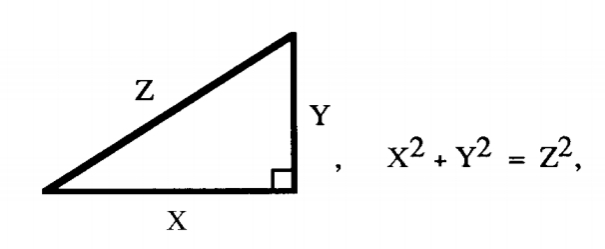
\includegraphics[width=10cm]{9.jpg}\\
			 % \caption{初}
		\end{figure}
	
		显然有$  (3,4,5)  $与$ (5,12,13) $等解.如何找全部整数解?等式$X^{2}+Y^{2}=Z^{2}$是齐次的,所以$ x=X/Z,y=Y/Z $就给出了圆$ C:(X^{2}+Y^{2}=1) \supset R^{2}$,它可以被参数化表示为:
		
		\begin{equation*}
			x=2 \lambda /\left(\lambda^{2}+1\right), y=\left(\lambda^{2}-1\right) /\left(\lambda^{2}+1\right),其中\lambda=x /(1-y)
		\end{equation*}
		
		
		所以下式可以给出所有解:
		
		
		\begin{equation*}
			X=2 \ell m, Y=\ell^{2}-m^{2}, Z=\ell^{2}+m^{2}\text { 其中 }\ell, m \in \mathbb{Z} \text { 互素 }
		\end{equation*}
	
	
		(若$ \ell,m $都是奇数,得到的$ X,Y,Z $值也可以各除以2).由于该等式为齐次,所以如果$ (X,Y,Z) $是一组解,那么$ (\lambda X,\lambda Y,\lambda Z) $也是一组解.
		
		
		在之前的几何教学中,我们已经对参数化有了相当的了解,并且通常我们都能很简单地判断参数化是否有效.而如果我们不是很了解参数化,我们可以通过下面的\textit{从定点出发的线性映射}来初步地理解:
	
	

		\begin{figure}[H]
		  \centering
		  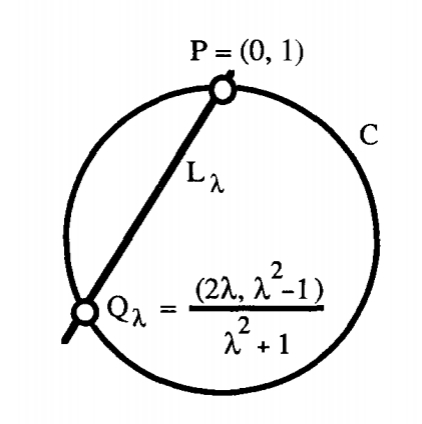
\includegraphics[width=6cm]{10.jpg}\\
		 % \caption{初}
		\end{figure}\par


		$ P=(0,1)\in C $,如果$\lambda \in Q$取任意值,那么穿过$ P $点斜率为$-\lambda$的直线$L_{\lambda}$与$ C $相交于另一点$Q_{\lambda}$.这种线性映射的映射结构会在以后的讨论中经常出现.
	
	\section{相似的例子}
		对于$ C:(2 X^{2} + Y^{2} =5 Z^{2}) $我们可以构造一个$ \mathbb{Z} \to C $的参数化的映射:
		
		\begin{equation*}
		x=\frac{2 \sqrt{5} \lambda}{1+2 \lambda^{2}}, \quad y=\frac{2 \lambda^{2}-1}{1+2 \lambda^{2}}
		\end{equation*}
		
		
		
		这样有助于我们理解C上所有实系数的点,而且和之前的例子没有本质上的区别.那么,如果是有理系数呢?
	
	
		\textbf{命题}\ 如果$ (a,b,c) \in \mathbb{Q} $满足$ 2a^{2}+b^{2}=5c^{2} $那么$ (a,b,c)=(0,0,0) $.
	
	
		\textbf{证明}\ 通过同时乘公分母与除以公因子,可以使得$ a,b,c $为整数,且他们不能同时为5的倍数.而如果$5\lvert a$且$ 5\lvert b $那么$ 25 \lvert c $,即$ 5 \lvert c $,这与上述题设矛盾.考虑$ a $和$ b $除以5的余数很容易得到矛盾:任何数的平方除以5后的余数只可能为0,1或4,即$2 a^{2}+b^{2}$除以5的余数只能是0+1,0+4,2+0,2+1,2+4,8+0,8+1以及8+4中的一个,而这些都不能写成$5 c^{2}$的形式.
	
	
		注意,这是一个完整的算数证明.
	\section{$\mathbb{Q}^{2}$中的圆锥曲线}
		$\mathbb{Q}^{2}$中的圆锥曲线是由二次方程$q(x,y)=ax^{2}+bxy+cy^{2}+dx+ey+f=0$给出的平面曲线.
	
	
		非退化的曲线有以下三种分类:
	
	
		1.椭圆$\dfrac{x^{2}}{a^{2}}+\dfrac{y^{2}}{b^{2}}=1$\indent
		2.抛物线$y=mx^{2}$\indent
		3.双曲线$\dfrac{x^{2}}{a^{2}}-\dfrac{y^{2}}{b^{2}}=1$
	
	
		此外,还有一些特殊情况:
	
	
		4.由$x^{2}+y^{2}=0$给出的单点.
	
	
		5.6.7.为三种类型方程给出的空集:5.$x^{2}+y^{2}=-1$ \indent  6.$x^{2}=-1$ \indent 7.$ 0=1 $.
		
		
		虽然这三种类型的方程都表示$R^{2}$上的空集,但是它们是不同的——例如考虑它们的复数解.
		
		
		8.一条直线:$ x=0 $.
		
		
		9.一对相交直线:$ xy=0 $.
		
		
		10.一对平行直线:$ x(x-1)=0 $.
		
		
		11.重合的直线:$x^{2}=0$.
		
		
		12.整个平面:$ 0=0 $.
	
	
	\section{射影平面$\mathbb{P}^{2}_{\mathbb{R}}$}
		\textbf{定义}
		\begin{equation*}
		\begin{aligned} \mathbb{P}^{2}_{\mathbb{R}}&= \mathbb{R}^{3} \text {中过原点的直线} \\ &=\{\text {比例} X : Y : Z\} \\ &=\left(\mathbb{R}^{3} \backslash\{0\}\right)/ \sim, \text { 其中 }(X, Y, Z) \sim(\lambda X, \lambda Y, \lambda Z), \lambda \in \mathbb{R} \backslash\{0\} \end{aligned}
		\end{equation*}
	
		(这里可以将$\mathbb{R}^{3}$推广到任意维的向量空间上)
	
	
	 	为了表示$ Z\neq0 $时的比例$ X:Y:Z $,可以设$x=\dfrac{X}{Z},y=\dfrac{Y}{Z}$,这样比例就相当于两个实数.换句话说,等价类$ (X:Y:Z) $有一个特殊的代表元$ (x:y:1) $.可是,在$ Z=0 $时,选择这种代表元的方式就无法实现了.这个讨论意味着$\mathbb{P}^{2}_{\mathbb{R}}$包含着一个$\mathbb{R}^{2}$,如图:
		\begin{figure}[H]
		  \centering
		  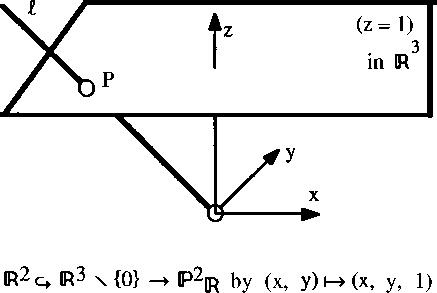
\includegraphics[width=10cm]{12.jpg}
		 % \caption{初}
		\end{figure}
	
		\vspace{-9mm}
		\begin{equation*}
		\mathbb{R}^{2} \hookrightarrow \mathbb{R}^{3} \backslash\{0\} \rightarrow \mathbb{P}^{2}_{\mathbb{R}} \text{由}(x, y) \mapsto(x, y, 1) \text{定义}
		\end{equation*}
		\vspace{5mm}
	
		$\mathbb{R}^{3}$中通过$ 0 $且不包含在平面($ Z=0 $)的直线都与平面($ Z=1 $)交于一点,这一点可以看做是等价类的代表元.而包含在平面($ Z=0 $) 中的直线与平面($ Z=1 $)无交点,所以他们不对应于$\mathbb{R}^{2}$中的点但对应于一个渐进方向,或者说对应于,$\mathbb{R}^{2}$中的一组平行线.所以可以认为$\mathbb{P}^{2}_{	\mathbb{R}}$是由$\mathbb{R}^{2}$和每组平行线方向上的无穷远点组成的.从这个角度来看,可以在$\mathbb{R}^{2}$中进行计算,通过某种渐进理论去猜想在无穷远点的情况,然后(如果必要的话),用齐次坐标去证明猜想.从$\mathbb{R}^{3}$中的直线来定义使之变得合理,因为这个定义平等地对待$\mathbb{P}^{2}_{\mathbb{R}}$上的所有点.
		
		
		变换群在整个几何中都是非常重要的,几何图形的性质要在一些变化类下保持不变才有意义.$\mathbb{R}^{2}$坐标中的仿射变换形式为$ T(x)=Ax+B $, 其中$x=(x,y)\in \mathbb{R}^{2}$,并且$ A $是一个$2\times2$的可逆矩阵,$ B $是一个平移向量;如果矩阵$ A $是正交矩阵,那么变换$ T $为欧式变换.每个非退化的曲线都可以通过欧式变换化成以上(1-3)的形式.
		
		
		$\mathbb{R}^{2}_{\mathbb{R}}$中的射影变化形式为$ T(x)=MX $,其中$ M $是一个$3\times3$的可逆矩阵.很容易理解这个变换在仿射片$\mathbb{R}^{2} \subset \mathbb{P}^{2}_{\mathbb{R}}$ 上的影响:作为一代部分定义的映射$\mathbb{R}^{2}\rightarrow \mathbb{R}^{2}$,这是一个分式线性变换
		
		\begin{equation*}
		\begin{pmatrix} x \\ y  \end{pmatrix}
		\rightarrow (A\begin{pmatrix} x \\ y\end{pmatrix}+B)/(cx+dy+e)
		\end{equation*}
	
		其中,
		\begin{equation*}
		M=\begin{pmatrix} A  & B \\ c  d &e\end{pmatrix}
		\end{equation*}
	
		当$ cx+dy+e=0 $时,这个变换无定义.
	\section{平面曲线的方程}
		非齐次二次多项式
		
		\begin{equation*}
				q(x,y)=ax^{2}+bxy+cy^{2}+dx+ey+f
		\end{equation*}
	
		对应齐次二次方程式
		
		\begin{equation*}
			Q(X,Y,Z)=aX^{2}+bXY+cY^{2}+dXZ+eYZ+fZ^{2}
		\end{equation*}
		
		这种对应关系很容易理解为菜谱,或者你可以把它看作是由以下方面给出的双射$Q  \longleftrightarrow q$,
		\begin{equation*}
			q(x,y)=Q(X/Z,Y/Z,1) \text{其中} x=X/Z,y=Y/Z,Z=1
		\end{equation*}
	
	
		反过来
		\begin{equation*}
			Q=Z^{2}q(X/Z,Y/Z)
		\end{equation*}
	
		平面曲线$C\subset \mathbb{P}^{2}$是由$ C:(Q(X,Y,Z)=0) $给出的曲线,其中$ Q $是齐次二次表达式;条件$ Q(X,Y,Z)=0 $在等价类上是良定义的,因为对任意的$\lambda \in \mathbb{R}, Q(\lambda X)=\lambda^{2}Q(X)$.
		
		
		\textbf{‘无穷远直线’与渐近方向}\ 
		$\mathbb{P}^{2}$中$ Z=0 $表示的点对应比例$ (X:Y:0) $,这些点形成了‘无穷远直线’$\mathbb{P}^{1}_{\mathbb{R}}=\mathbb{R} \cup \{ \infty \}$(因为$(X:Y)\mapsto X/Y$定义了一个双射$P^{1}_{R} \rightarrow R \cup \{ \infty \}$)
		
		
		 $\mathbb{P}^{2}$中的直线是由$ L:(aX+bY+cZ=0) $定义的,并且$ L $通过$(X,Y,0)\Longleftrightarrow aX+bY=0$. 在仿射坐标中,相同的直线是由$ ax+by+c=0 $给出的,从而使所有$a : b$比率相同的直线在无穷远处通过同一点. 这就是所谓的“平行线在无穷远处相遇”.
		
		
		\textbf{例子}:
		
		
		(a)\ $\mathbb{R}^{2}$中的双曲线($\frac{x^{2}}{a^{2}}-\frac{y^{2}}{b^{2}}=1$)对应于$\mathbb{P}^{2}_{\mathbb{R}}$中的C:($\frac{X^{2}}{a^{2}}-\frac{Y^{2}}{b^{2}}=Z^{2}$);很明显,在$(b,±a,0)\in \mathbb{P}^{2}_{\mathbb{R}}$的两点满足$ (Z=0) $,这两个点对应于双曲线的渐近线.
		
		
		注意,在$\mathbb{P}^{2}_{\mathbb{R}}$的仿射片($X\neq 0$)中, 仿射坐标是$ u=Y/X,v=Z/X $,这样C就变成了椭圆($\frac{u^{2}}{b^{2}}+v^{2}=\frac{1}{a^{2}}$).
		
		
		(b)\ $\mathbb{R}^{2}$中的抛物线($y=mx^{2}$)对应于$\mathbb{P}^{2}_{\mathbb{R}}$中的$C:(YZ=mX^{2}$);在单点$ (0,1,0) $处满足$ Z=0 $. 因此在$\mathbb{P}^{2}$中,“抛物线的两个分支在无穷远处相遇”.
	
	
	\section{$\mathbb{P}^{2}$中平面曲线的分类}
		k是一个特征不为2的域,回想二次型线性代数的两个结果:
		
		
		\textbf{命题(A)}\ 有天然的双射$\{ \text{二次齐次多项式} \}=\{\text{二次型}k^{3} \to k \} \longleftrightarrow \{k^{3}\text{上的对称双线性型}\}$,并且可以由下式给出:
		\begin{equation*}
		aX^{2}+2bXY+cY^{2}+2dXZ+2eYZ+fZ^{2} \longleftrightarrow \begin{bmatrix} a & b &d \\ b & c &e\\ d & e & f\end{bmatrix}
		\end{equation*}
		如果相应的双线性形式是非退化的,则二次型是非退化的,就是说,这个矩阵是非奇异的.
		
		
		\textbf{定理(B)}\ $ V $是$ k $上的向量空间,$Q:V\to k\text{是二次型},\text{则存在一组}V\text{的基使}Q=\varepsilon_{1}x^{2}_{1}+\varepsilon_{2}x^{2}_{2}+\cdots\varepsilon_{n}x^{2}_{n}$,其中$\varepsilon_{i}\in k$.(格拉姆-施密特正交化证明了这一点)
		
		
		\textbf{推论}\ 在适当的坐标系中,$\mathbb{P}^{2}_{\mathbb{R}}$中的任何圆锥曲线都是下列情况之一:
		
			
		(1)非退化曲线, $C:(X^{2}+Y^{2}-Z^{2}=0)$;
		
		
		(2)空集, $(X^{2}+Y^{2}+Z^{2}=0)$;
		
		
		(3)交叉线对, $(X^{2}-Y^{2}=0)$;
		
		
		(4)一个点$(0,0,1)$, $(X^{2}+Y^{2}=0)$;
		
		
		(5)重叠线$(X^{2}=0)$;
		
		
		(可以将$\mathbb{P}^{2}_{\mathbb{R}}$整个平面由$ (0=0) $给出.)
		
	
		\textbf{证明}\ 任何实数$\varepsilon$ 是0或$\pm \sqrt{a}$, 因此我们只需要考虑定理中$\varepsilon=0$或$\pm1$的Q. 另外, 由于我只对轨迹$ (Q = 0) $感兴趣, 所以我可以把Q乘以-1,这将立即得出给定的列表.
		
		
		关于这个推论有两点: 首先, 列表比$ (1.3) $中的要短得多: 例如, $ (1.3) $的3个非退化情况(椭圆、抛物线、双曲线)都对应情况(1). 在射影情形下不区分交叉和平行的线对这两种情况. 其次, 从一般代数学原理推导出以上几种情况更简单一点.
	\section{曲线参数化}
		设$ C $是$\mathbb{P}^{2}_{\mathbb{R}}$中的非退化的非空二次曲线. 由推论$ 1.6 $, 取新的坐标$ (X+Z, Y, Z-X) $, $ C $与曲线$(XZ=Y^{2})$在投影上等价, 这个曲线的参数化是
	
		\begin{equation*}
		\begin{array}{l}{\Phi : \mathbb{P}^1_{\mathbb{R}}\quad \longrightarrow \quad C \subset \mathbb{P}^{2}_{\mathbb{R}}} \\ {(U : V) \quad\longmapsto\quad  \left(U^{2} : UV : V^{2}\right)}\end{array}
		\end{equation*}

		\textbf{备注}
		
		
	 	1. 相反的映射$\Psi: C\longrightarrow P^{1}_{R}$由$(X:Y:Z)\longmapsto(X:Y)=(Y:Z)$给出;如果 $Y \neq 0$,就按左边的比例定义, 如果 $Z \neq 0$, 就按右边的比例定义.在后面要介绍的术语中,$\Phi$ 和$\Psi$ 是变换的逆同构.
	
	
		2.任意非空的非退化二次曲线默认为投影等价于$(XZ=Y^{2})$;在特征不为2的域中,这在练习5中是合理的(对特征为2的域感兴趣的读者应该把这个作为非退化二次曲线的定义).
	\section{2个变量的齐次型}
		设$ F(U, V) $为关于$ U, V $的d次非零齐次多项式, 系数在固定的域k内
		
		\begin{equation*}
		F(U,V)=a_{d}U^{d}+a_{d-1}U^{d-1}V+...+a_{i}U^{i}V^{d-i}+...a_{0}V^{d}
		\end{equation*}
		
		F有一个与之相关的单变量非齐次多项式:
		
		\begin{equation*}
			f(u)=a_{d}u^{d}+a_{d-1}u^{d-1}+...+a_{i}u^{i}+...a_{0}
		\end{equation*}
		
		显然对于$ \alpha \in k $,有
		\begin{equation*}
		f(\alpha )=0 \Leftrightarrow (u-\alpha)|f(u)\Leftrightarrow (U-\alpha V)|F(U,V)\Leftrightarrow F(\alpha,1)=0
		\end{equation*}
		
		所以$ f $的零点对应于$ F $在$\mathbb{P}^{1}$上除点$ (1,0) $的零点,而点$ (1,0) $对应于‘点$\alpha =\infty$’.$ F $在无穷远处有一个零点是什么意思?
		
		\begin{equation*}
			F(1,0)=0\Leftrightarrow a_{d}=0\Leftrightarrow deg f<d
		\end{equation*}
		
		现在定义$ F $在$\mathbb{P}^{1}$上零点的重数为
		
		
		(i) $\alpha \in k$在f中的重数;
		
		
		(ii)如果$ (1,0) $是零点,重数为$ d-deg f $.
		
		
		所以$ F $在$ (\alpha,1) $处的零点重数是$ (U-\alpha V) $除F的最大幂, 在$ (1,0) $处是$ V $除$ F $的最大幂.
		
	
		\textbf{命题}\ 设$ F(U,V) $是$ U,V $的$ d $次的非零齐次多项式, 那么F在$mathbb{P}^{1}$上最多有$ d $个零点;此外,如果$ k $是代数闭域, 那么$ F $在$mathbb{P}^{1}$上恰好有$ d $个零点, 前提是这些数要用上面定义的乘法来计算.
		
		
		\textbf{证明}\ 令$m_{\infty}$为$ F $在$ (1,0) $处的零点重数;然后根据定义, $d-m_{\infty}$是非齐次多项式$ f $的次数, 然后这个命题可以归结为一个众所周知的事实,即单变量多项式最多有$ deg f $个根.
		
		
		注意,在代数封闭域上, $ F $将分解为线性形式$\lambda_{i}=(a_{i}U+b_{i}V)$的乘积$F=\Pi\lambda_{i}^{m_{i}}$,用这种方法处理,点$ (1,0) $ 对应于形式$\lambda_{\infty}=V$,并且与所有其他点处于相同的地位.
	\section{贝祖定理的简单情况}
		贝祖定理指出, 如果$ C $和$ D $是次数为$ deg C=m, deg D=n $的平面曲线,并且
		
		
		(i)域是代数闭的;(ii)交点个数按重数来计数;(iii) 我们在$\mathbb{P}^{2}$中计算, 所以考虑无穷远处的交点. 则$ C $和$ D $的交点个数为$ mn $. 见[Fulton,p.112 ]有自成一体的证明.在本节中, 将在其中一条曲线是直线或二次曲线的情况下证明.
		
		
		\textbf{定理}\ 设$L\subset \mathbb{P}^{2}_{k}$是一条直线($C\subset \mathbb{P}^{2}_{k}$是一条非退化二次曲线), $D\subset \mathbb{P}^{2}_{k}$是由$D:(G_{d}(X,Y,Z)=0)$ 定义的一条曲线, 其中$ G $是关于$ X, Y, Z $中的$ d $次齐次多项式. 假定 $ L $不包含于 $ D $($ C $ 不包含于$ D $); 则$ L $与$ D $的交点个数$\# \{L\cap D\}$小于等于$ d $ ($\# \{C\cap D\}$小于等于$ 2d $).
		
		
		事实上, 对于交点的重数有一个自然的定义, 使得对于用重性计数的交点的个数, 不等式仍然成立, 如果k是代数闭的, 那么等式成立.
		
		
		\textbf{证明}\ $\lambda$ 为线性形式, 由 $\lambda=0$ 给出的一条直线$L\subset P^{2}_{k}$, 将其按下面方式参数化
		
		\begin{equation*}
			X=a(U,V), Y=b(U,V), Z=c(U,V)
		\end{equation*}
	
		其中$ a,b,c $是$ U,V $的线性形式.例如, 如果$\lambda=\alpha X+\beta Y+\gamma Z$, 且$\gamma \neq 0$, 那么$ L $可以参数化为$ X=U,Y=V, Z=-\dfrac{\alpha}{\gamma}U-\dfrac{\beta}{\gamma}V$. 类似的, 正如$ (1.7) $中证明的, 非退化曲线可以参数化为$ X=a(U,V), Y==b(U,V),Z=c(U,V) $.其中$ a,b,c $是$ U,V $中的二次型,这是因为$ C $是$(XZ=Y^{2})$的射影变换, 它的参数化方式为$ (X,Y,Z)=(U^{2},UV,v^{2})$,所以$ C $是
		
		\begin{equation*}
		 \begin{bmatrix} X \\Y\\ Z\end{bmatrix}=M\begin{bmatrix} U^{2} \\UV\\ V^{2}\end{bmatrix}
		\end{equation*}
	
		其中$ M $是$ 3\times3 $非奇异矩阵.
	
		\begin{figure}[H]
		  \centering
		  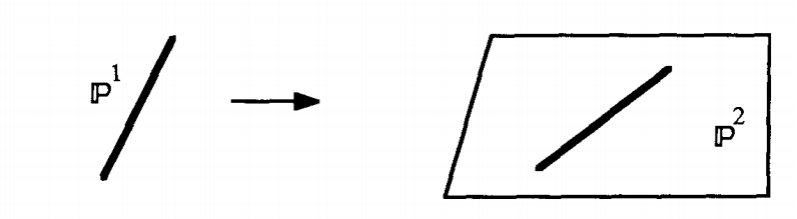
\includegraphics[width=7cm]{1811.jpg}参数化直线\\
		  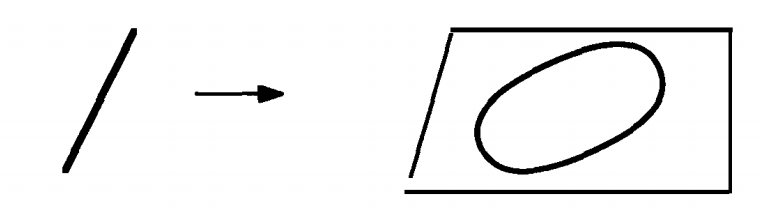
\includegraphics[width=7cm]{1822.jpg}参数化二次曲线\\
		 % \caption{初}
		\end{figure}
	
		然后通过$F(U:V)=G_{d}(a(U,V),b(U,V),c(U,V))=0$求出$ (U:V) $的比值, 求出$ L $(或曲线$ C $)与$ D $的交点.但$ F $是关于$ U,V $的$ d $(或为$ 2d $)次的齐次多项式, 因此可参考$ (1.8) $得出结果.

	\section{推论}
		如果$P_{1},...,P_{5} \in \mathbb{P}^{2}_{R}$是任意四点不共线的5个点,那么就至多存在一条圆锥曲线穿过$P_{1},...,P_{5}$.
		
		
		\textbf{证明} 用反证法假设$C_{1}$和$C_{2}$是两条不相同的圆锥曲线使得
		\begin{equation*}
		C_{1} \cap C_{2} \supset \{ P_{1},...,P_{5}\}
		\end{equation*}
	
		$C_{1}$是非空的因此它是非退化的,那么,由$ (1.7) $,它投影地等价于参数化的圆锥曲线
		
		\begin{equation*}
		C_{1}=\{(U^{2},UV,V^{2}) \mid (U,V)\in P^{1}\}
		\end{equation*}
	
		由(1.9),$C_{1} \subset C_{2}$.那么,如果$Q_{2}$与$C_{2}$相等,那么$Q_{2}(U^{2},UV,V^{2})\equiv 0$对于任何$(U,V)\in P^{1}$成立,并且通过简单计算(如习题$ 1.6 $)就可以看出$Q_{2}$是$(XZ-Y^{2})$的倍数,这与$C_{1}\ne C_{2}$相矛盾.
		
		
		现在假设$C_{1}$是退化的,由(1.6)可知,它是一组线对或是一条线,而且很明显有
		
		\begin{equation*}
		C_{1}=L_{0}\cup L_{1},C_{2}=L_{0}\cup L_{2}
		\end{equation*}
	
		其中$ L_{1} L_{2} $是不同的线.那么$C_{1}\cap C_{2}=L_{0}\cup (L_{1}\cap L_{2})$
	\begin{figure}[H]
	  \centering
	  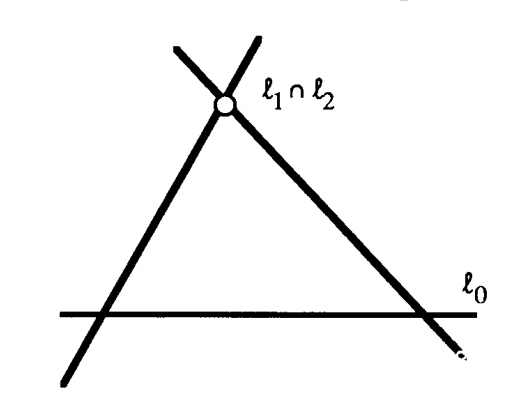
\includegraphics[width=6cm]{19.jpg}
	 % \caption{初}
	\end{figure}
		因此,$P_{1}...P_{5}$中的4点在$P_{0}$上,自相矛盾.
		
	\section{所有二次曲线的空间}
		$S_{2}=\{R^{3} \text{中的二次型}\}=\{3\times3\text{对称矩阵}\}\cong R^{6}$, 如果$Q\in S_{2}$, $Q=aX^{2}+2bXY+\cdots fZ^{2}$;对于$P_{0}=(X_{0},Y_{0},Z_{0})\in P^{2}_{R}$, 考虑到$P_{0}\in C:(Q=0)$的关系,这是形式$Q(X_{0},Y_{0},Z_{0})=aX^{2}_{0}+2bX_{0}Y_{0}+\cdots fZ_{0}=0$, 对于固定的$P_{0}$, 这是关于$(a,b,\cdots f)$ 的线性方程. 所以$S_{2}(P_{0})=\{Q\in S_{2}|Q(P_{0})=0\}\cong R^{5}\subset S_{2}=R^{6}$是一个5维的超平面.
		
		
		对于$P_{1},\cdots P_{n}\in P^{2}_{R}$, 类似地定义$S_{2}(P_{1},\cdots P_{n})=\{Q\in S_{2}|Q(P_{i})=0  i=1,\cdots n\}$;所以可以得到关于$ Q $的6个系数$(a,b,\cdots f)$的$ n $个线性方程. 这得出了以下结果:
		
		
		\textbf{命题}\ $dimS_{2}(P_{1},\cdots P_{n})\geq6-n$.
		
		
		如果$P_{1},\cdots P_{n}$能都满足以些条件,我们也可以期望等式成立, 更准确地说应该是:
		
		
		\textbf{推论}\ 如果$n\leq5$并且$P_{1},\cdots P_{n}$中任意4点不共线,则$dimS_{2}(P_{1},\cdots P_{n})=6-n$.
		
		
		\textbf{证明}\ 推论1.10表明, 如果n = 5, $dim S_{2}(P_{1},\cdots P_{n})\leq1$,给出了这种情况的证明.如果$n\leq4$, 然后我可以加入点$P_{n+1},\cdots,P_{5}$ 并且保持没有4个点共线的条件, 由于每个点最多增加一个线性条件, 所以$1=dimS_{2}(P_{1},\cdots P_{5})\geq dimS_{2}(P_{1},\cdots P_{n})-(5-n)$.
		
		
		请注意, 如果给定6个点$P_{1},\cdots P_{6}$, 可能存在在一条圆锥曲线同时包含这6个点, 也可能不存在.
		
	\section{两条圆锥曲线的交点}
		\begin{figure}[H]
		  \centering
		  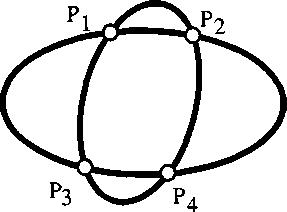
\includegraphics[width=5cm]{20.jpg}\\
		 % \caption{初}
		\end{figure}
		正如我们上面所看到的, 两个二次曲线经常会在4个点相交;相反, 根据推论$ (1.11) $, 给定4个点$P_{1},\cdots P_{4}\in P^{2}$, 在适当条件下$S_{2}(P_{1},\cdots P_{4})$是一个二维向量空间,因此选择$S_{2}(P_{1},\cdots P_{4})$的一组基$Q_{1},Q_{2}$给出了2条二次曲线$C_{1},C_{2},$ 使得$C_{1}\cap C2=\{P^{1},\cdots P^{4}\}$.
		
		
		这里还有许多非退化曲线多重交点的可能性:
		\begin{figure}[H]
		  \centering
		  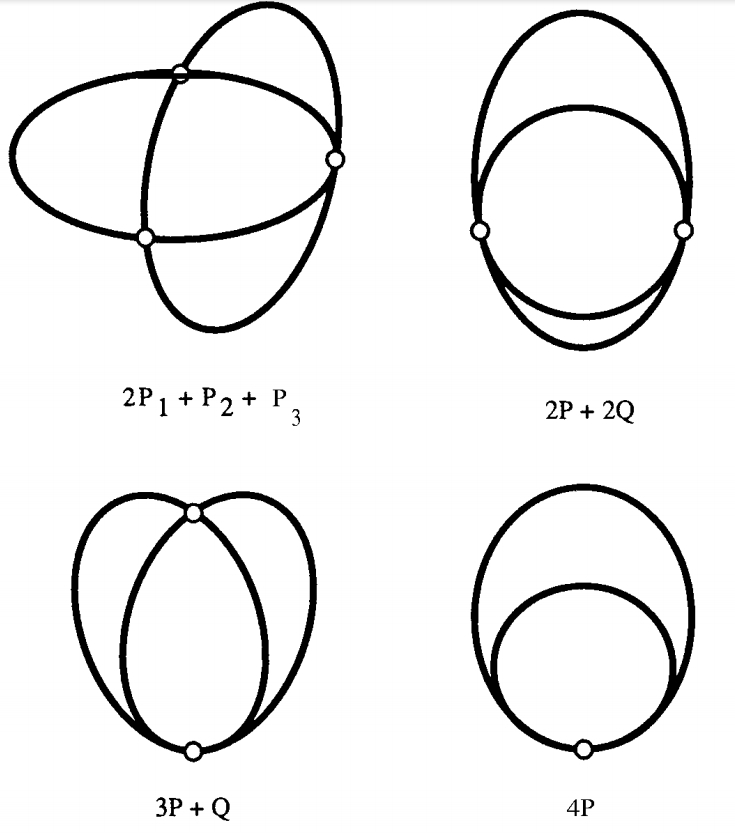
\includegraphics[width=8cm]{21.jpg}
		 % \caption{初}
		\end{figure}
	
	
		\textit{有关合适的方程式见\textit{练习1.9a}}
		
		\section{退化的圆锥曲线族}
		\textbf{定义}\ \textit{圆锥曲线族}是一类满足以下特点的齐次多项式:
		
		\begin{equation*}
		C_{(\lambda, \mu)} :\left(\lambda Q_{1}+\mu Q_{2}=0\right)
		\end{equation*}
		
		其中的每一个元素都是一条由参数$(\lambda, \mu)$线性控制的平面圆锥曲线.类似于我们在$\mathbb{P}^{1}$上做的那样,我们可以用一个比例$(\lambda : \mu)$来代表对应的平面圆锥曲线.
		
		
		如示例中,只有当$(\lambda : \mu)$为一个特殊值时,平面圆锥曲线$C_{(\lambda, \mu)}$才是退化的.事实上,如果将二次齐次多项式$Q$对应的$3 \times 3$对称矩阵的行列式记作$\operatorname{det}(Q)$,那么显然有
		\begin{equation*}
		C_{(\lambda, \mu)} \text {是退化的} \Longleftrightarrow \operatorname{det}\left(\lambda Q_{1}+\mu Q_{2}\right)=0
		\end{equation*}
		
		
		将对称矩阵$Q_{1}$和$Q_{2}$表述的条件记作:
		\begin{equation*}
		F(\lambda, \mu)=\operatorname{det}\left|\lambda\left[\begin{array}{ccc}{a} & {b} & {d} \\ {b} & {c} & {e} \\ {d} & {e} & {f}\end{array}\right]+\mu\left[\begin{array}{ccc}{a^{\prime}} & {b^{\prime}} & {d^{\prime}} \\ {b^{\prime}} & {c^{\prime}} & {e^{\prime}} \\ {d^{\prime}} & {e^{\prime}} & {f^{\prime}}\end{array}\right]\right|=0
		\end{equation*}
		
		
		那么就可以注意到$F(\lambda, \mu)$是一个对于$\lambda, \mu$的三次齐次多项式,那么我们就可以对$F$应用$(1.8)$的结论:
		
	
		\textbf{命题} \ 假设$C_{(\lambda, \mu)}$是在$\mathbb{P}^{2}_{k}$上的一族圆锥曲线,并且这一族圆锥曲线至少有一个非退化的(因此$F(\lambda, \mu)$不总是0),那么这一族中最多有三个退化的圆锥曲线.另外,如果有$k=\mathbb{R}$,那么这一族最少有一个退化的圆锥曲线.
		
		
		\textbf{证明} \ 一个三次齐次多项式的零点个数$\leq 3$.而在$\mathbb{R}$上,它最少有一个零点.

	\section{一些实例}
		令$P_{1} \ldots P_{4}$是$\mathbb{P}^{2}_{\mathbb{R}}$上任意三个不共线的四点,则经过这四点的圆锥曲线族$C_{(\lambda, \mu)}$有三个退化的元素,即线对$L_{12}+L_{34}, L_{13}+L_{24}, L_{14}+L_{23}$,其中$L_{ij}$是过$P_{i},P_{j}$的直线:
		\begin{figure}[H]
		  \centering
		  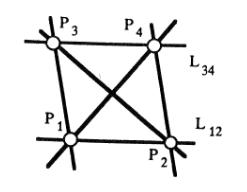
\includegraphics[width=5cm]{22.jpg}
		 % \caption{初}
		\end{figure}
	
	
		{然后,我们假设这一族圆锥曲线是由$Q_{1}=Y^{2}+r Y+s X+t$和$Q_{2}=Y-X^{2}$生成的,并寻找$P_{1} \ldots P_{4}$这四个交点.}
		
		\begin{figure}[H]
		  \centering
		  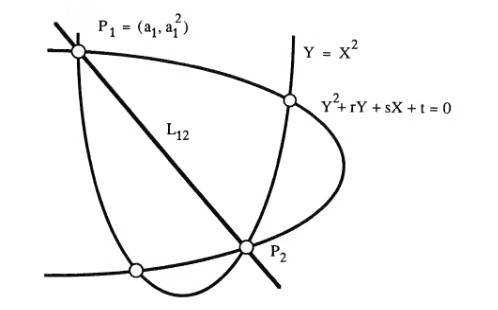
\includegraphics[width=8cm]{23.jpg}
		 % \caption{初}
		\end{figure}
	
	
		通过下列步骤可解:
		
		
		$(1)$找出三个比例$(\lambda : \mu)$使得$C_{(\lambda, \mu)}$是退化的圆锥曲线.根据上文,这意味着我们需要找到三次齐次多项式的三个根
		\begin{equation*}
			\begin{aligned} F(\lambda, \mu) &=\operatorname{det}\left|\lambda\left[\begin{array}{ccc}{0} & {0} & {s / 2} \\ {0} & {1} & {r / 2} \\ {s / 2} & {r / 2} & {t}\end{array}\right]+\mu\left[\begin{array}{ccc}{-1} & {0} & {0} \\ {0} & {0} & {1 / 2} \\ {0} & {1 / 2} & {0}\end{array}\right]\right| \\ &=-\frac{1}{4}\left(s^{2} \lambda^{3}+\left(4 t-r^{2}\right) \lambda^{2} \mu-2 r \lambda \mu^{2}-\mu^{3}\right) \end{aligned}
		\end{equation*}
		
		
		$(2)$从退化的圆锥曲线中分出2条作为线对(这意味着解两个四次方程).
		
		
		$(3)$这四个交点$P_{i}$就是线的交点.
		
		
		这个步骤给出了利用伽罗瓦理论解四次方程的一个几何解释:设$k$是一个域,而$f(X)=X^{4}+r X^{2}+s X+t \in k[X]$是一个四次多项式.则两条抛物线$C_{1}$和$C_{2}$相交于四个点$P_{i}=\left(a_{i}, a_{i}^{2}\right)(i = 1\ldots4)$,而$a_{i}$是$f$的四个根.
		
		
		则直线$L_{ij}=P_{i} P_{j}$由下式给出:
		\begin{equation*}
			L_{ij} :\left(Y=\left(a_{i}+a_{j}\right) X-a_{i} a_{j}\right)
		\end{equation*}
		
		而可约的圆锥曲线$L_{12}+L_{34}$由下式给出:
		\begin{equation*}
			Y^{2}+\left(a_{1} a_{2}+a_{3} a_{4}\right) Y+\left(a_{1}+a_{2}\right)\left(a_{3}+a_{4}\right) X^{2}+s X+t=0
		\end{equation*}
	
		这是由$Q_{1}-\left(a_{1}+a_{2}\right)\left(a_{3}+a_{4}\right) Q_{2}=0$推出的.因此,使圆锥曲线$\lambda Q_{1}+\mu Q_{2}$退化为线对的3个比例$(\lambda : \mu)$的值为:
		
		\begin{equation*}
			-\left(a_{1}+a_{2}\right)\left(a_{3}+a_{4}\right),-\left(a_{1}+a_{3}\right)\left(a_{2}+a_{4}\right),-\left(a_{1}+a_{4}\right)\left(a_{2}+a_{3}\right)
		\end{equation*}
		根是这三个数的三次方程被称为与四次方程对应的\textit{辅三次方程};这可以通过初等对称函数的理论计算得到;因此这是一个极具可操作性的步骤.而在另一方面,上面给出的概要优雅地给出了仅有三阶行列式的辅三次方程的一个推导.
		
	\section*{练习1}
		\subsection{考虑通过$ (-1,-2) $的直线,将二次曲线$C:(x^{2}+y^{2}=5)$参数化.并找出$(x^{2}+y^{2}=5)$的所有有理解.}
			解:由
				\begin{equation*}
				  \left\{
				   \begin{aligned}
				 x^{2}+y^{2} &=5 \\
				 y+2= &k(x+1)\\
				   \end{aligned}
				   \right.
				\end{equation*}
			得
				\begin{equation*}
				  \left\{
				   \begin{aligned}
				  x &=\frac{-k^{2}+4k+1}{1+k^{2}} \\
				  y &=\frac{2k^{2}+2k-2}{1+k^{2}}\\
				   \end{aligned}
				   \right.
				\end{equation*}
			
			
			若(a,b)是$(x^{2}+y^{2}=5)$的解, 则$ (-a,-b),(-a,b),(a,-b) $也是$(x^{2}+y^{2}=5)$的解. 所以不妨找$a>0, b>0$的有理解, 由上述参数化知,$ (x,y) $是有理点$\Leftrightarrow k\in Q$, $x>0, y>0\Leftrightarrow \frac{2}{\sqrt{5}+1}<k<\sqrt{5}+2$
			
		\subsection{p是质数,猜想$x^{2}+y^{2}=p$有有理解的充要条件,证明你的猜想. }
			(若$x^{2}=a(mod \ p)$有解,称a是模p 的二次剩余.数论里的一个基本结论, -1是模$ p $ 的二次剩余当且仅当$ p=2 $或$ p=1mod16 $. )
			
			解:猜想$ p=2 $或$ p=1mod 4 $
			
			
			 $x^{2}+y^{2}=p$有有理解, $x=\frac{a}{c},y=\frac{b}{c},\Leftrightarrow a^{2}+b^{2}=pc^{2}$有整数解.
			
			$"\Rightarrow"$ \ a是模$ p $的二次剩余$\Leftrightarrow a^{\frac{p-1}{2}}=1(mod \ p)$, 显然1一定是模$ p $的二次剩余(因为$a^{\frac{p-1}{2}}=1(mod \ p)$),所以$x^{2}=1(mod \ p)$有解. 若$ (a,b,c) $满足$a^{2}+b^{2}=pc^{2}$, 则一定满足$a^{2}+b^{2}=pc^{2}(mod \ p)$. 因为一定存在$ a $, 使$a^{2}=1(mod \ p)$,所以一定存在$ b $使$b^{2}=-1(mod \ p)$, 得$ p=2 $或$ p=1mod4 $.
			
			$"\Leftarrow"$ \ $ p=2 $时, $1^{2}+1^{2}=2$, 所以$ (1,1) $是 $x^{2}+y^{2}=2$的有理解.
			
			$ p=1mod  4 $时,$ p=4k+1 , k \in Z$
			$a^{2}=1,0(mod 4),b^{2}=1,0(mod 4)$, 所以$a^{2}+b^{2}=pc^{2}=1,2(mod 4)$,
			即$a^{2}+b^{2}=pc^{2}=4k^{2}+1,4k^{2}+2$, 而$pc^{2}=(4k+1)c^{2}=4kc^{2}+c^{2}=c^{2}(mod 4)=1,2$,
		\subsection{证明1.3中的陈述:仿射变换可以将任何一条圆锥曲线变为1-12中的形式.}
		
		
			解答:使用线性变换$ x \mapsto Ax $把$ax^{2}+bxy+cy^{2}$的部分转换为$\pm x^{2} \pm y^{2},\pm x^{2}$或0的形式;然后再通过配方将尽可能多的线性部分消除
		\subsection{对1.3中的仿射圆锥曲线和1.6中的射影圆锥曲线进行详细的比较}
			解答:(1).非退化圆锥曲线,对应椭圆、抛物线、双曲线;
			
			
			(2).空集,对应1.3中4、5、6三种情况;
			
			
			(3).线对,对应7、8、9三种情况;
			
			
			(4).单点,对应4;
			
			
			(5).双线,对应10;
			
			
			另外,视情况,可认为整个射影平面对应0=0;
			
			
			将1.3的多项式所对应的矩阵化为只由1和-1组成的对角形式的矩阵,则1.6中从上到下的式子分别对应:
			$\begin{bmatrix}
			    1&0&0\\
			    0&1&0\\
			    0&0&-1\\
			\end{bmatrix}
			\begin{bmatrix}
			    1&0&0\\
			    0&1&0\\
			    0&0&1\\
			\end{bmatrix}
			\begin{bmatrix}
			    1&0&0\\
			    0&-1&0\\
			    0&0&0\\
			\end{bmatrix}
			\begin{bmatrix}
			    1&0&0\\
			    0&1&0\\
			    0&0&0\\
			\end{bmatrix}
			\begin{bmatrix}
			    1&0&0\\
			    0&0&0\\
			    0&0&0\\
			\end{bmatrix}$
		\subsection{$ k $为特征值不为2的任意数域,$ V $是$ k $上的三维向量空间,$ Q:V \to k $是一个V上的非退化的二次型.请证明如果$ 0 \ne e_{1} \in V $满足$ Q(e_{1} )=0 $那么V有基底$e_{1},e_{2},e_{3}$使得$ Q(x_{1} e_{1} + x_{2} e_{2} + x_{3} e_{3} )= x_{1} x_{3} +a x_{2}^{2}$.}
			解答:设一对称双线性型满足:
				$\varphi(\alpha,\beta)=\alpha 'A \beta$ (之后简写为($\alpha,\beta$))
				
				
				$ Q(e_{1} )=0 \Rightarrow \varphi (e_{1},e_{1} )=0 $
				
				
				$\varphi(e_{1},e_{3})=1$
				
				
				则$Q(x_{1} e_{1}+x_{2} e_{2}+x_{3} e_{3} )= \varphi (x_{1} e_{1}+x_{2} e_{2}+x_{3} e_{3},x_{1} e_{1}+x_{2} e_{2}+x_{3} e_{3} )
				=2 x_{1} x_{2}(e_{1},e_{3} )+2 x_{1} x_{3}+x_{2}^{2}(e_{2},e_{2} )+ x_{3}^{2}(e_{3},e_{3})+2 x_{2} x_{3}(e_{2},e_{3})$
				
				
				下证$\exists e_{2} \ne 0$使得$(e_{1},e_{2} )=0;(e_{2},e_{3} )=0;(e_{2},e_{2})\ne 0$
				
				
				首先
				\begin{equation*}
				\left\{\begin{aligned}\left(e_{1}, e_{2}\right) &=0 \\\left(e_{3}, e_{2}\right) &=0 \end{aligned} \Rightarrow\left\{\begin{array}{l}{\left(x_{1} y_{1} z_{1}\right) A e_{2}=0} \\ {\left(x_{3} y_{3} z_{3}\right) A e_{2}=0}\end{array}\right.\right. \text{有解}
				\end{equation*}
			%	下面两行在一个大括号里
			%	($e_{1}$,$e_{2}$)=0\\
			%	($e_{3}$,$e_{2}$)=0
			%	
			%	$\Rightarrow$
			%	
			%	下面两行在一个大括号里
			%	($x_{1}$$y_{1}$$z_{1}$)A$e_{2}$=0
			%	($x_{3}$$y_{3}$$z_{3}$)A$e_{2}$=0
			%	有解
				
				$\begin{bmatrix}
				    (x_{1}y_{1}z_{1})A\\
				    (x_{3}y_{3}z_{3})A\\
				\end{bmatrix}$
				秩$\le 2$,解空间维数$\ge 1$
				
				
				$(e_{1},e_{2})=0,(e_{3},e_{2})=0$
				
				
				若$(e_{2},e_{2})=0,e_{2}=0$得出矛盾
				
				
				故$e_{2}\ne 0$
				
				
				可得$Q(x_{1} e_{1} + x_{2} e_{2}+x_{3} e_{3} )=2 x_{1}x_{3}+x_{2}^{2} (e_{2},e_{2} )+ x_{3}^{2}(e_{3},e_{3} )$
				
				
				$e_{3}'=\lambda e_{1}+\mu e_{3}$(令$\mu=1$)$\Rightarrow e_{3} '=- \frac{e_{2}e_{3}}{2} e_{1}+e_{3}$
				
				
				最后再取$e_{1}'= \frac{1}{\sqrt{2}} e_{1},e_{3} ''= \frac{1}{\sqrt{2}} e_{3}'$
				
				
				得证
		\subsection{设k是一个至少有4个元素的域,$C:(XZ=Y^{2})\supset P^{2}_{k}$.证明:如果$ Q(X,Y,Z) $是在C上为0的二次型,则$ Q=\lambda(XZ-Y^{2}) $.}
			解答:带入特殊点即可,可得Q所对应的矩阵为
			$\begin{bmatrix}
			    0&0&\lambda\\
			    0&-2\lambda&0\\
			    \lambda&0&0\\
			\end{bmatrix}$
		\subsection{在$ \mathbb{R}^{3} $上,考虑$ A:(Z = 1) $和$ B:(X = 1) $两个平面,一条过原点的直线交平面$ A $于$ (x,y,1) $,交平面$ B $于 $ (1,\dfrac{y}{x},\dfrac{1}{x}) $.考虑由$(x, y) \mapsto\left(y^{\prime}=\dfrac{y}{x}, z^{\prime}=\dfrac{1}{x}\right)$定义的映射 ,当原象为\\
		(1)直线族$ ax = y + b $ (其中$ a $是定值而$ b $是变量)\\
		(2)圆$(x-1)^{2}+y^{2}=c$其中c是变量(注意$ c $的取值)\\
		时,考虑它的象.并且指出当映射或逆映射没有定义时的情况.}
		
			解答:
			(1)设参数$ t $,则有$ ax = y + b $交$ A:(Z = 1) $于$ (t,at-b,1) $,参考题干给出的映射,直线在$ B:(X = 1) $上为$ (1,\dfrac{at-b}{t},\dfrac{1}{t}) $.则映射下的象为$ bz' = -y' + a $.显然,映射和逆映射总有定义.
			
			
			(2)设参数$ \theta $,取$ x = 1 + c\cos\theta,y = c\sin\theta $,参考题干给出的映射,有$ y' = \dfrac{c\sin\theta}{1+c\cos\theta},z' = \dfrac{1}{1+c\cos\theta} $.则映射下的象为$ y'^{2} = (c^{2}-1)z'^{2} +2z' -1 $,当$ c<1 $时是椭圆,当$ c = 1 $时是抛物线,当$ c>1 $时是双曲线.当映射没有定义时,有$ x = 0 $,即圆与$ A:(Z = 1) $的交点为$ (0,y,1) $;当逆映射没有定义时,有$ x = \infty $,即圆与$ A:(Z = 1) $ 的交点为$ (\infty,y,1) $.
		
		\subsection{$ P_{1},\cdots P_{4} $是$ \mathbb{P}^{2} $上任意三点不共线的四点.证明:存在一个仿射坐标系使得这四个点的坐标分别为$ (1,0,0),(0,1,0),(0,0,1) $和$ (1,1,1) $,设$ P_{5} = (a,b,c)$是这四个点以外的第五个点,找到所有经过这五个点的圆锥曲线并给出推论1.10和引理1.11的另外一个证明.}
		
			解答:设$ P_{1},\cdots P_{4} $的坐标为$ (x_{i},y_{i},1) ,i = 1,\cdots 4$.考虑$ (x_{i},y_{i},1) ,i = 1,\cdots 4$到$ (1,0,0),(0,1,0),(0,0,1),(1,1,1) $的仿射变换$ Ax +b = y $,则有
			
			
			$\left(\begin{array}{lll}{a_{11}} & {a_{12}} & {a_{33}} \\ {a_{21}} & {a_{22}} & {a_{23}} \\ {a_{31}} & {a_{32}} & {a_{33}}\end{array}\right)\left(\begin{array}{l}{x_{1}} \\ {y_{1}} \\ 1\end{array}\right)+\left(\begin{array}{l}{b_{1}} \\ {b_{2}} \\ {b_{3}}\end{array}\right)=\left(\begin{array}{c}{1} \\ {0} \\ {0}\end{array}\right)$
			
			
			$\left(\begin{array}{lll}{a_{11}} & {a_{12}} & {a_{33}} \\ {a_{21}} & {a_{22}} & {a_{23}} \\ {a_{31}} & {a_{32}} & {a_{33}}\end{array}\right)\left(\begin{array}{l}{x_{2}} \\ {y_{2}} \\ 1\end{array}\right)+\left(\begin{array}{l}{b_{1}} \\ {b_{2}} \\ {b_{3}}\end{array}\right)=\left(\begin{array}{c}{0} \\ {1} \\ {0}\end{array}\right)$
			
			
			$\left(\begin{array}{lll}{a_{11}} & {a_{12}} & {a_{33}} \\ {a_{21}} & {a_{22}} & {a_{23}} \\ {a_{31}} & {a_{32}} & {a_{33}}\end{array}\right)\left(\begin{array}{l}{x_{3}} \\ {y_{3}} \\ 1\end{array}\right)+\left(\begin{array}{l}{b_{1}} \\ {b_{2}} \\ {b_{3}}\end{array}\right)=\left(\begin{array}{c}{0} \\ {0} \\ {1}\end{array}\right)$
		
		
			$\left(\begin{array}{lll}{a_{11}} & {a_{12}} & {a_{33}} \\ {a_{21}} & {a_{22}} & {a_{23}} \\ {a_{31}} & {a_{32}} & {a_{33}}\end{array}\right)\left(\begin{array}{l}{x_{4}} \\ {y_{4}} \\ 1\end{array}\right)+\left(\begin{array}{l}{b_{1}} \\ {b_{2}} \\ {b_{3}}\end{array}\right)=\left(\begin{array}{c}{1} \\ {1} \\ {1}\end{array}\right)$
			
			
			由于$ P_{1},\cdots P_{4} $任意三点不共线,所以$ \left(\begin{array}{llll}{x_{1}} & {x_{2}} & {x_{3}}& {x_{4}} \\ {y_{1}} & {y_{2}} & {y_{3}}& {y_{4}} \\ 1 & 1 & 1& 1\end{array}\right) $是非奇异的,因此可以解得$ A $和$ b $,则存在符合题意的仿射坐标系.
			
			
			已知,圆锥曲线在仿射变换下仍然为圆锥曲线,因此我们只需要在仿射坐标系下进行证明.显然,存在圆锥曲线族经过$ (1,0,0),(0,1,0),(0,0,1) $和$ (1,1,1) $,设为$ A $,若存在一条圆锥曲线$ C $经过这四个点及另外一点,则有$ C \in A $,将这样的$ C $上的所有点的集合记为$ P $并且有$ P \not = R^{2},P \not = \emptyset $.此时,若$ P_{5} \in P$,则有且仅有一条圆锥曲线经过$ P_{1},\cdots P_{5} $,否则则没有这样的圆锥曲线.
		\subsection{(1.12)给出了两个圆锥曲线相交的所有可能性.写下每种可能性对应的方程,并找出对应的曲线族中的奇异曲线.(使用对称矩阵可能会比坐标系简单许多)}
		
			解答:因为圆锥曲线在仿射变换下不变,因此不妨取其中一条圆锥曲线为$ x^{2}+y^{2} = 1 $,此时易得:
			
			
			(1)$ 2x^{2}+\dfrac{y^{2}}{2} = 1 $
			
			
			(2)$ 2x^{2}+\dfrac{y^{2}}{2} = \dfrac{\sqrt{2}}{2} $
			
			
			(3)$ 2x^{2}+y^{2} = 1 $
			
			
			(4)$ (x+\dfrac{1}{2})^{2}+y^{2} = 1 $
			
			
			(5)$ (x+\dfrac{1}{2})^{2}+y^{2} = \dfrac{1}{4} $
		
		
		
		
		
		\subsection{(西尔维斯特行列式)设k为代数闭域, U为二次齐次多项式, Y为三次齐次多项式, (按(1.8)节的定义):}
		\begin{equation*}
		\begin{array}{l}{q(U,V)=a_{0}U^{2}+a_{1}UV+a_{2}V^{2}} \\ {c(U,V)=b_{0}U^{3}+b_{1}U^{2}V+b_{2}UV^{2}+b_{3}V^{3}}\end{array}
		\end{equation*}
		证明$ q $和$ c $有一个公共的零点$(\eta:\tau)\in \mathbb{P}^{1}$当且仅当
		\begin{equation*}
		\operatorname{det}\left|\begin{array}{ccccc}{a_{0}} & {a_{1}} & {a_{2}} & {0} & {0} \\ {0} & {a_{0}} & {a_{1}} & {a_{2}} & {0} \\ {0} & {0} & {a_{0}} & {a_{1}} & {a_{2}} \\ {b_{0}} & {b_{1}} & {b_{2}} & {b_{3}} & {0} \\ {0} & {b_{0}} & {b_{1}} & {b_{2}} & {b_{3}}\end{array}\right|=0
		\end{equation*}
		
			证明:记\[Res(q,c)=
			det\left|\begin{array}{cccccc}
			  a_{0} &  a_{1} & a_{2}&0 &0\\
			    0 & a_{0} &  a_{1} & a_{2}&0 \\
			    0 & 0 &a_{0} &  a_{1} & a_{2}\\
			    b_{0} &  b_{1} & b_{2}& b_{3} &0\\
			    0 &  b_{0} &  b_{1} & b_{2}& b_{3}
			\end{array}\right|
			\]
			必要性:证法一:若$ (1,0) $是公共解, 则$a_{0}=b_{0}=0$, 所以$ Res(q,c)=0 $.
			
			
			若$ (1,0) $不是公共解, 则
			\begin{equation*}
			  \left\{
			   \begin{aligned}
			   q(x) &=a_{0}x{2}+a_{1}x+a_{2} \\
			  c(x) &=b_{0}x^{3}+b_{1}x^{2}+b_{2}x+b_{3}\\
			   \end{aligned}
			   \right.
			\end{equation*}
			有公共解$\frac{\eta}{\tau}=x_{0}$.
			
			  所以 $ q(x),c(x) $可分解成
			  \begin{equation*}
			  \left\{
			   \begin{aligned}
			   q(x) &=q_{1}(x)(x-x_{0}) \\
			  c(x) &=c_{1}(x)(x-x_{0})\\
			   \end{aligned}
			   \right.
			   \end{equation*}
			   其中$q_{1}(x)$为一次多项式,$ c_{1}(x)$为二次多项式, 设为$q_{1}(x)=u_{0}x+u_{1}, c_{1}(x)=v_{0}x^{2}+v_{1}x+v_{2}$. 所以
			   \begin{equation*}
			   c_{1}(x)q(x)=q_{1}(x)c(x) \tag{$*$}
			 \end{equation*}
			比较(*)式多项式两边的系数可得
			\begin{equation*}
			  \left\{
			   \begin{aligned}
			   a_{0}v_{0} &=b_{0}u_{0} \\
			  a_{1}v_{0}+a_{0}v_{1} &= b_{0}u_{1}+b_{1}u_{0}\\
			    a_{2}v_{0}+a_{1}v_{1}+a_{0}v_{2} &= b_{1}u_{1}+b_{2}u_{0}\\
			    a_{2}v_{1}+a_{1}v_{2} &= b_{3}u_{0}+b_{2}u_{1}\\
			    a_{2}v_{2} &=b_{3}u_{1}
			   \end{aligned}
			   \right. \tag{$**$}
			   \end{equation*}
			   由于$q(x)\neq0,c(x)\neq0$, 所以$q_{1}(x)\neq0,c_{1}(x)\neq0$,即$(v_{0},v_{1},v_{2},-u_{0},-u_{1})\neq0$.
			
			
			   (**)对应的齐次方程有非零解$(v_{0},v_{1},v_{2},-u_{0},-u_{1})$, 所以\[
			det\left|\begin{array}{cccccc}
			  a_{0} &  0 & 0&b_{0} &0\\
			    a_{1} & a_{0} &  0 & b_{1}& b_{0} \\
			    a_{2} & a_{1} &a_{0} &  b_{2} & b_{1}\\
			    0 &  a_{2} & a_{1}& b_{3} &b_{2}\\
			    0 &  0 &  a_{2} & 0& b_{3}
			\end{array}\right|=0
			\]
			进而$ Res(q,c)=0 $.
			
			
			证法二:如果$ q,c $有公共解,则$U^{2}q, UVq, V^{2}q, Uc, Vc $有公共零解$(\eta:\tau)\in P^{1}$,其中
			\begin{equation*}
			  \left\{
			   \begin{aligned}
			   U^{2}q &=a_{0}U^{4}+a_{1}U^{3}V+a_{2}U^{2}V^{2} \\
			  UVq &= a_{0}U^{3}V+a_{1}U^{2}V^{2}+a_{2}UV^{3}\\
			    V^{2}q &= a_{0}U^{2}V^{2}+a_{1}UV^{3}+a_{2}V^{4}\\
			   Uc &= b_{0}U^{4}+b_{1}U^{3}V+b_{2}U{2}V^{2}+b_{3}UV^{3}\\
			    Vc &=b_{0}U^{3}V+b_{1}U^{2}V^{2}+b_{2}UV^{3}+b_{3}V^{4}
			   \end{aligned}
			   \right.
			\end{equation*}
			   所以$S((\eta:\tau))=k_{1}U^{4}+k_{2}U^{3}V+k_{3}U^{2}V^{2}+k_{4}UV^{3}+k_{5}V^{4}$同构于$R^{4}$,
			
			   所以5个向量$(a_{0},a_{1},a_{2},0,0),(0,a_{0},a_{1},a_{2},0), (0,0,a_{0}, a_{1},a_{2}),(b_{0}, b_{1},b_{2},b_{3},0), (0,b_{0},b_{1},b_{2},b_{3})$是线性相关的,即得$ Res(q,c)=0 $.
			
			   充分性:$ Res(q,c)=0 $, 则齐次方程
			   \begin{equation*}
			  \left\{
			   \begin{aligned}
			   a_{0}x_{1}+b_{0}x_{4} &=0 \\
			  a_{1}x_{1}+a_{0}x_{2}+b_{1}x_{4}+b_{0}x_{5} &=0\\
			    a_{2}x_{1}+a_{1}x_{2}+a_{0}x_{3}+b_{2}x_{4}+b_{1}x_{5} &=0\\
			    a_{2}x_{2}+a_{1}x_{3}+b_{3}x_{4}+b_{2}x_{5} &=0\\
			    a_{2}x_{3}+b_{3}x_{5} &=0
			   \end{aligned}
			   \right.
			   \end{equation*}
			   有非零解,设为$(v_{0},v_{1},v_{2},-u_{0},-u_{1})\neq0$, 代入上面的方程即可得到(**)式.
			
			   由
			   \begin{equation*}
			     \begin{aligned}
			   &q(x) =a_{0}x^{2}+a_{1}x+a_{2} \\
			 & c(x) =b_{0}x^{3}+b_{1}x^{2}+b_{2}x+b_{3}\\
			 & q_{1}(x) =u_{0}x+u_{1}\\
			 &  c_{1}(x) =v_{0}x^{2}+v_{1}x+v_{2}
			   \end{aligned}
			  \end{equation*}
			  可以得到(*)式, 且$deg q_{1}(x)<2,deg c_{1}(x)<3$
			
			  当$a_{0},b_{0}$不全为0时,不妨假设$a_{0}\neq0$, 则$ deg q(x)=2 $, 由(*), $q(x)|q_{1}(x)c(x),$ 反设$ q(x),c(x) $无公共零点, 则$ (q(x),c(x))=1 $, 所以$q(x)|q_{1}(x)$, 则$ deg q(x) $小于等于$deg q_{1}(x)<2$, 矛盾, 所以$ q(x),c(x) $有公共零点,设为$\alpha$ , 则$(\alpha,1)$是$ q(U,V),c((U,V)  $的公共零解.
			
			  当$a_{0},b_{0}$全为0时,易得$ q(U,V),c((U,V) $有公共零解$ (1,0) $.
		\subsection{把习题$ 1.10 $的结果推广到$ U,Y $为任意$ n $和$ m $次的两种形式中.}
			设k为代数闭域,f,g分别是关于U,V的n次,m次齐次形式, 
			\begin{equation*}
			\begin{aligned} f(U, V) &=a_{0} U^{n}+a_{1} U^{n-1} V+\cdots+a_{n-1} U V^{n-1}+a_{n} V^{n} \\ g(U, V) &=b_{0} U^{m}+b_{1} U^{m-1} V+\cdots+b_{m-1} U V^{m-1}+a_{m} V^{m} \end{aligned}
			\end{equation*}
			f和g有一个公共的零点$(\eta:\tau)\in P^{1}$当且仅当
			\[
			det\left|\begin{array}{ccccccccc}
			  a_{0} &  a_{1} & \cdots &a_{n} &0 &\cdots & 0 & 0&0\\
			    0 & a_{0} &  a_{1} & \cdots &a_{n}&0&\cdots & 0 &0\\
			    \cdots & \cdots &\cdots & \cdots& \cdots& \cdots& \cdots& \cdots \cdots\\
			  0&0&  \cdots& 0&\cdots & a_{0} &a_{1} & \cdots & a_{n}\\
			    b_{0} &  b_{1} &  \cdots& \cdots& b_{m} &0&\cdots & 0 & 0\\
			    0 &  b_{0} &  b_{1} &  \cdots&  \cdots& b_{m}& 0&  \cdots&0\\
			     \cdots & \cdots &\cdots & \cdots& \cdots& \cdots& \cdots& \cdots \cdots\\
			   0& \cdots &\cdots &0 &  b_{0} &  b_{1} &  \cdots&  \cdots& b_{m}
			
			\end{array}\right|=0
			\]

\chapter{三次曲线和群定律}
	\section{三次曲线参数化的例子}正如二次曲线那样,一些平面三次曲线可以参数化:
	
	
		\textbf{结点三次曲线} \ $C:(y^{2}=x^{3}+x^{2})\subset R^{2}$是映射 $\phi:R^{1}\rightarrow R^{2} , t\longmapsto(t^{2}-1,t^{3}-t) $的象.
		
		\textbf{尖点三次曲线} \ $C:(y^{2}=x^{3})\subset R^{2}$是映射 $\phi:R^{1}\rightarrow R^{2} , t\longmapsto(t^{2},t^{3}) $的象.
		
		\begin{figure}[h]
		  \centering
		  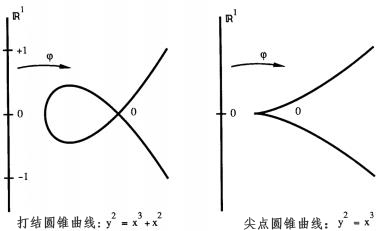
\includegraphics[width=10cm]{27.jpg} \\
		 % \caption{初}
		\end{figure}
		
		\textit{想想图像曲线和映射的奇点, 这些例子会贯穿整个课程, 所以花点时间来处理这些方程;见\textit{练习2.1-2}.}

	\section{曲线$(y^{2}=x(x-1)(x-\lambda))$没有有理参数化}
		参数化曲线很好; 例如, 如果您对丢番图问题感兴趣, 您可以期望一个表达式给出所有有理值点, 如(1.1)所示.(1.1)的参数化形式为$ x = f(t), y = g(t) $, 其中$ f $和$ g $是有理函数,即两个多项式的商.
		
		\textbf{定理} \ $ k $是一个特征不为2的域, $\lambda\in k$且$\lambda\neq0,1,f,g\in k(t)$是有理函数, 满足$(f^{2}=g(g-1)(g-\lambda)$, 则$f,g\in k$.
		
		
		这相当于说不存在任何由有理函数给出的非常数映射$R^{1}\rightarrow C: (y^{2}=x(x-1)(x-\lambda))$.
		
		
		定理的证明是在$ k(t) $中利用$ k(t) $是唯一分解环$ k[t] $的分式域的事实.
		
		
		\textbf{证明} \ $ k[t] $是唯一分解环, 设$f=r/s,  r,s\in k[t]$且互素, $g=p/q,  p,q\in k[t]$且互素, 代入 $(f^{2}=g(g-1)(g-\lambda)$得
		$\dfrac{r^{2}}{s^{2}}=\dfrac{p}{q}(\dfrac{p}{q}-1)(\dfrac{p}{q}-\lambda)$, 除去公分母后得, $r^{2}q^{3}=s^{2}p(p-q)(p-\lambda q)$, 因为$ r $和$ s $是互素的, 右边的因子$s^{2}$一定整除$q^{3}$. 同理,因为$ p$ 和 $q $是互素的, 左边的因子$q^{3}$一定整除$s^{2}$.所以,$s^{2}|q^{3}$ 且$q^{3}|s^{2}$, 所以$s^{2}=aq^{3}$, 其中$a\in k$($ a $是$ k[t] $中的单位,所以$a\in k$).
		
		
		可得$aq=(\dfrac{s}{q})^{2}$是$ k[t] $中的平方形式. 并且$r^{2}=ap(p-q)(p-\lambda q)$, 所以考虑分解到素元的因式分解, 存在非零常数$b,c,d\in k $ 使$bp,c(p-q),d(p-\lambda q)$是$ k[t] $中的平方形式. 下面如果能证明$ p, q $是常数, 那么$ r, s $也是, 定理得证. 为了证明$ p, q $是常数, 设$ K $是$ k $的代数闭包; 那么$p,q\in K[t]$满足以下引理的条件.

	\section{引理}
		K是一个代数闭域, $p,q\in K[t]$互素,假设4个不同的线性组合($\lambda p+\mu q$, 4个不同的比例$(\lambda:\mu)\in P^{1}_{k}$)为$ K[t] $中的平方形式. 那么$p,q\in K$.
		
		
		\textbf{证明} \ (费马无穷递降法)将$ p,q $替换成$ p'=ap+bq,q'=cp+dq $, 其中$a,b,c,d\in K$并且$ad-bc\neq 0$,不会影响定理的假设和结论, 因此我可以假设4 个给定的平方形式是$p,p-q,p-\lambda q,q$. 那么$p=u^{2},q=v^{2}$, 并且$u,v\in K[t]$互素, 则$max\{deg u,deg v\}$小于$max\{deg p,deg q\}$. 假设$max\{deg p,deg q\}$大于0, 并且是满足引理条件的$ p,q $中次数最小的, 那么$p-q=u^{2}-v^{2}=(u-v)(u+v)和p-\lambda q=u^{2}-\lambda v^{2}=(u-\mu v)(u+\mu v)$(其中$\mu=sqrt{\lambda}$)是$ K[t] $中的平方形式. 所以根据$ u,v $互素的形式,可得每个$u-v,u+v,u+\mu v,u-\mu v$都是平方形式. 这与$ max\{deg p,deg q\} $的极小性矛盾. 所以$max\{deg p,deg q\}=0, p,q\in K.$
	\section{线性系统}
		记$S_{d}$={$ (X,Y,Z) $的$ d $次型}(这个形式是齐次多项式),任意元素$F \in S_{d}$可以唯一地写成
		\begin{equation*}
		F=\sum a_{ijk} X^{i}Y^{j}Z^{k},a_{ijk} \in k
		\end{equation*}
		i+j+k=d;这意味着$S_{d}$是一个$ k $上的向量空间,它有基底
		\begin{center}
		$Z^{d}$\\
		$Z^{d-1}X  \quad Z^{d-1}Y$\\
		..            ..\\
		$X^{d-1}Z  \quad X^{d-2}YZ  ..  \quad Y^{d-1}Z$\\
		$X^{d}\quad X^{d-1}Y  \quad X^{d-2}Y^{2}\quad   ..  \quad Y^{d}$\\
		\end{center}
		特别的,$dimS^{d}$=
		$\begin{pmatrix}
		     d+2  \\
		      2
		\end{pmatrix}$
		.对于$P_{1},...P_{n} \in P^{2}$,令
		\begin{equation*}
		S_{d}(P_{1},..P_{n})=\{F_{E}S_{d}|F(P_{i})=0,i=1,2,...n\} \subset S_{d}
		\end{equation*}
		对于每个条件$ F(P_{i})=0 $,(或者更精确一点,$ F(X_{i},Y_{i},Z_{i}=0,P_{i}=(X_{i}:Y_{i}:Z_{i})) $
		是$ F $上的线性条件,使得$S_{d}(P_{1},..P_{n})$是一个维数$\geq\left(\begin{array}{c}{d+2} \\ {2}\end{array}\right)-n$的向量空间.
	\section{引理}
		设$ k $是一个无限域,$F \in S_{d}$.
		
		
		(i)记$L\subset \mathbb{P}^{2}_{k}$为一条直线,如果在$ L $上$F\equiv 0$,那么$ F $由$ L $的方程在$ k[X,Y,Z] $上是可分的.这是说,$ F=H·F' $成立,当$ H $是$ L $的方程且$F'\in S_{d-1}$
		
		
		(ii)记$C\subset \mathbb{P}^{2}_{k}$是一条非空非退化的圆锥曲线,如果在$ C $上$ F \equiv 0 $,,那么$ F $由$ C $的方程在$ k[X,Y,Z] $上是可分的.这是说,$ F=Q·F' $成立,当$ Q $是$ C $的方程且$F' \in S_{d-1}$
		证明.(i)通过坐标变换,我们可以假定$ L=X $,那么对于任意的$F \in S_{d}$,存在唯一一个表达式$F=X· F'_{d-1} +G(Y,Z)$:只需把所有含$ X $的单项式集中到第一个被加数里,剩下的就必然只有含$ Y,Z $的多项式.现在有在$ L $上$F \equiv 0 \Leftrightarrow$在$ L $上$G \equiv 0\Leftrightarrow G(Y,Z)=0$. 最后一步是由于(1.7):如果$ G(Y,Z) \ne 0 $,那么它在$\mathbb{P}^{1}_{k}$上至多有$ d $个零点,然而如果$ k $是无限域,那么对于$\mathbb{P}^{1}_{k}$也一样.
		
		
		(ii)通过坐标变换,$Q=XZ-Y^{2}$.现在证明对任意$F\in S_{d}$,都存在唯一一个表达式$ F=Q·F'_{d-2}+A(X,Z)+YB(X,Z) $:如果用$ (XZ-Q) $来代替$Y^{2}$,那么剩下的部分$ Y $的次数就一定不大于1,故是$ A(X,Z)+YB(X,Z) $的形式.正如在(1.8)中,$ C $是一个由$X=U^{2},Y=UV,Z=V^{2}$参数化的圆锥曲线,使得
		\begin{equation*}
		\begin{split}
		C\text{上}F\equiv0&\Leftrightarrow C\text{上}A(U^{2},V^{2})+UVB(U^{2},V^{2})\equiv0\\
		&\Leftrightarrow A(U^{2},V^{2})+UVB(U^{2},V^{2})=0\in k[U,V]\\
		&\Leftrightarrow A(X,Z)=B(X,Z)=0
		\end{split}
		\end{equation*}
		
		分开考虑$ A(U^{2},V^{2})+UVB(U^{2},V^{2}) $的奇次项和偶次项最后一个等式可以得到最后一个等式.证毕.
		
		
		\textit{练习2.2给出了明确的零点定理的相似例子.}
		
		\textbf{推论}\ 令$L:(H=0)\subset \mathbb{P}^{2}_{k}$为一条直线(另外的$C:(Q=0) \subset \mathbb{P}^{2}_{k}$是一条非退化圆锥曲线);假设给定点$P_{1},P_{2} ... P_{n} \in P^{2}_{k}$,考虑$S_{d}(P_{1},P_{2} ... P_{n}),d$已给定.那么
		
		(i)如果$P_{1},P_{2} ... P_{a} \in L, P_{a+1},P_{a+2} ... P_{n} \notin L$,且$ a>d $,那么
		
		
		\quad $S_{d}(P_{1},P_{2} ... P_{n} )=H·S_{d-1}(P_{a+1},P_{2} ... P_{n})$
		
		(ii)如果$P_{1},P_{2} ... P_{a} \in C, P_{a+1},P_{a+2} ... P_{n} \notin C$,且$ a>2d $,那么
		
		
		\quad $S_{d}(P_{1},P_{2} ... P_{n} )=Q· S_{d-2}(P_{a+1},P_{2} ... P_{n})$
		
		
		证明:如果F是一个d次齐次多项式,曲线$ D:(F=0) $与$ L $相交于$P_{1}...P_{a}$当$ a>d $,那么由(1.8),就一定有$L\subset D$,使得由引理可知$ F=H·F $;由于$P_{a+1} ,...., P_{n} \notin L,显然F \in S_{d-1}(P_{a+1} ... P_{n})$.同理可得(ii)的结论.证毕.
	\section{命题}
		令k是一个无限域,$P_{1} ... P_{8} \in \mathbb{P}^{2}_{k}$是两两不同的点,如果这8点中没有任意两点共线,而且没有任意7点在同一个非退化圆锥曲线上,那么
		\begin{equation*}
		dimS_{3}(P_{1}...P_{8})=2
		\end{equation*}
		
		
		\textbf{证明}\ (2.6)的证明分几种情况.
		
		
		\textbf{大多数情况}\ 没有任意3点共线,没有任意6点共圆锥曲线.这是一般的位置情况.
		
		
		假设$dim S_{3}(P_{1}...P_{8})\ge 3$,然后令$P_{9},P_{10}$是直线$L=P_{1} P_{2}$.那么
		\begin{equation*}
		dim S_{3}(P_{1}...P_{10})\ge dim S_{3}(P_{1} ... P_{8} )-2 \ge 1
		\end{equation*}
		
		
		所以有$0 \ne F \in S_{3} (P_{1} ... P_{10} )$.由定理$ 2.5 $,$F=H·Q,Q \in S_{2} (P_{3} ... P_{8} )$.现在可以得出矛盾:如果$ Q $是非退化的那么$P_{3} ... P_{8}$是共圆锥曲线的,然而如果$ Q $是线对或二重线,那么它们中至少3点共线.
		\begin{figure}[H]
		  \centering
		  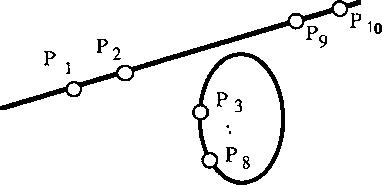
\includegraphics[width=8cm]{32.jpg}
		 % \caption{初}
		\end{figure}
	
	
		\textbf{第一退化情况}\ 设$P_{1} P_{2} P_{3} \in L$是共线的,令$ L:(H=0) $.令$P_{9}$是$ L $上的第四个点,那么由定理2.5,
		\begin{equation*}
		S_{3}(P_{1} ... P_{9} )=H· S_{2}(P_{4} ... P_{8} )
		\end{equation*}
		
		
		同样,由于$P_{4}...P_{8}$是共线的,由1.9,$dim S_{2}(P_{4} ... P_{8} )=1$,并且$dim S_{3}(P_{1} ... P_{9} )=1$,这意味着$dim S_{3}(P_{1} ... P_{8})\le 2$
		
		
		\textbf{第二退化情况}\ 设$P_{1} ... P_{6} \in C$是共圆锥曲线的,$ C:(Q=0) $是一个非退化圆锥曲线.那么选择区别于$P_{1} ... P_{6}$的$P_{9} \in C$,由定理2.5,
		\begin{equation*}
		S_{3}(P_{1} ... P_{9} )=Q· S_{1} (P_{7},_{8} )
		\end{equation*}
	
	
		线$L= P_{7} P_{8}$是唯一的,所以$S_{3}(P_{1}...P_{9})$是由$ QL $限制的一维空间,因此$dim S_{3}(P_{1} ... P_{8})\le 2$.证毕.
	\section{定理}
		$C_{1} C_{2}$是两条圆锥曲线,它们的交点是9个两两不同的点,$C_{1} \cap C_{2} ={ P_{1} ... P_{9} }$.那么圆锥曲线$ D $如果通过$P_{1} ... P_{8}$,也必然穿过$P_{9}$.
		
		
		\textbf{证明}\ 如果$P_{1} ... P_{9}$中的4个点在一条线$ L $上,那么$C_{1} C_{2}$的每一条都会与$ L $相交于4个点以上,因此就包含直线$ L $这与$C_{1}\cap C_{2}$的假设矛盾.同样的,不能有7个点共圆锥曲线.因此满足了2.6的假设,所以
		\begin{equation*}
		dim S_{3}\left(P_{1} \ldots P_{8}\right)=2
		\end{equation*}
		这意味着$C_{1},C_{2}$的等式$F_{1},F_{2}$构成了$S_{3}(P_{1} ... P_{8} )$的基.因此$ D:(G=0) $,其中G=$\lambda$$F_{1}$+$\mu$$F_{2}$.现在$F_{1},F_{2}$在$P_{9}$上退化,因此$ G $也一样.证毕.
	\section{平面三次曲线的群论}
		假设$ k \subset C $是$ C $的子域,$ F \in k[X,Y,Z] $是一个定义了一个非空平面曲线$ C $的三次型,$C:(F=0) \subset \mathbb{P}^{2}_{k}$.假定$ F $满足以下两条性质:
		
		
		(a)\ $ F $是不可约的(这样$ C $就不会包含一条直线或圆锥曲线);
		
		
		(b)\ 对于任意一点$ P \in C $,都存在唯一一条$L \subset \mathbb{P}^{2}_{k}$使得$ P $是$F|_{L}$的重根.
		
		
		几何上,条件(b)要求$ C $是非奇异的,$ L $指的是切线$L=T_{P} C$(见\textit{练习2.3}).
		
		
		固定任意一点$ O \in C $,进行下列构造:
		
		
		\textbf{构造}\ 
		\begin{minipage}[t]{0.9\linewidth}
			(i)对$ A \in C $,令$\overline{A}$为$ C $与$ OA $的第三个交点;\\
			(ii)对于$A,B\in$C,记$ R $为$ AB $与$ C $的第三个交点,定义$A+B=\overline{R}$.
		\end{minipage}
		
		\textbf{定理}\ 结合性是这里的关键.
		
		
		(I)需证明加法和逆运算是良定义的.如果$ P,Q $是$ C $上任意两点,那么$ P \ne Q $,这样$L=PQ\subset P^{2}_{k}$是唯一确定的,不然由假设(b)知$ P=Q $,那么有唯一一条直线$L\subset \mathbb{P}^{2}_{k}$使得$ P $ 是$F|_{L}$的重根;在另一种情况下,$F|_{L}$是有两个变量的三次型,有两个$ k $上的零点.因此它分为3个线性因式的乘积,故无一例外的,第三个交点$ R $是良定义的而且在k内有坐标.注意$ P=Q,P=R,Q=R,P=Q=R $都是可以的.这在代数上与$F|_{L}$有多个零点一致,在几何上与切线和回折点一致.
		
		
		\begin{figure}[H]
		  \centering
		  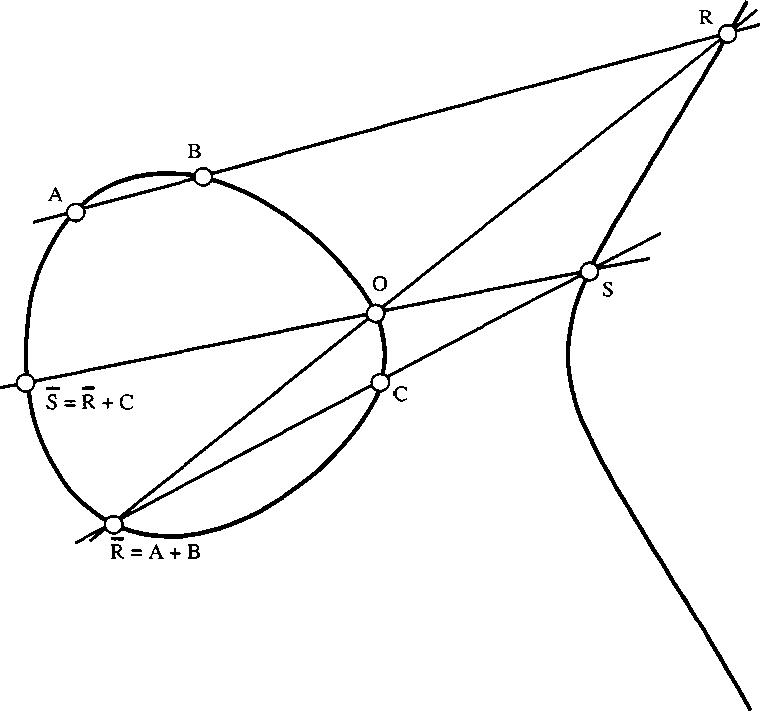
\includegraphics[width=10cm]{34.jpg}
		 % \caption{初}
		\end{figure}
		(II)验证零元$ O $点是符合零元条件的:$OA\overline{A}$是共线的,$ O+A $由$ L=OA $得到第三个交点$\overline{A}$,则同一条线$L=O\overline{A}$得到$ A $,得证.
		
		
		(III)$ A+B=B+A $显然.
		(IV)先由(i)定义点$\overline{O}$:令$ L $为使得$ O $是$F|_{L}$重根的直线,定义$\overline{O}$是$ L $与$ C $的第三个交点.那么显然对任意$ A \in C $,$\overline{O} A$的第三个交点都是$ A  $的逆.
	\section{}
		现在,我们给出一个“足够普遍”的情况下的结合律的证明:假设$ A,B,C $是三次曲线$ C $上的三点,而$(A+B)+C=\overline{S}$的构造用到了四条直线(如上一节图):
		\begin{equation*}
			L_{1}:ABR,L_{2}:RO\overline{R},L_{3}:C\overline{R}S,L_{4}:SO\overline{S}
		\end{equation*}
	
		$(B+C)+A=\overline{T}$的构造则用到了另外四条直线:
		
		\begin{equation*}
			M_{1}:BCQ,M_{2}:QO\overline{Q},M_{3}:A\overline{Q}T,M_{4}:TO\overline{T}
		\end{equation*}
		我们需要证明$\overline{S}=\overline{T}$,显然,只需要证明$S=T$即可.考虑三次曲线:
		\begin{equation*}
		D_{1}=L_{1}+M_{2}+L_{3} \text { 和 }D_{2}=M_{1}+L_{2}+M_{3}
		\end{equation*}
		由构造可知,
		\begin{equation*}
		C \cap D_{1}=\{A, B, C, O,R, \overline{R}, Q, \overline{Q}, S\}
		\end{equation*}
		\begin{equation*}
		C \cap D_{2}=\{A, B, C, O,R, \overline{R}, Q, \overline{Q}, T\}
		\end{equation*}
		已知,$ A, B, C, O,R, \overline{R}, Q, \overline{Q}, S $这九个点都是独立的,三次曲线$ C $ 和 $ D_{1} $满足推论2.7的条件,因此,$ D_{2} $ 一定经过$ S $,而这当且仅当$S=T$时成立.
		
		
		完成这个证明有很多方法,其中最彻底的证明给出了考虑多交点的两条曲线的交点的真实处理方法,而对应推论2.7的证明是Max Noether的引理.
		
	\section{}
		在这里,我们给出一个利用连续性的证明,这个证明将用到$ k \in \mathbb{C} $这个事实.对曲线$ C $考虑对应的复曲线$C_{\mathbb{C}} \subset \mathbb{P}^{2}_\mathbb{C}$,即当$ (X:Y:Z) $在复数域上时仍然有$ F(X,Y,Z)=0 $.而如果结合律在复曲线$ C_{\mathbb{C}} $上成立,那么显然在曲线$ C $ 上也处处成立.因此,我们不妨假设$ k = \mathbb{C} $.
		
		\textbf{引理}\ (i)$ A+B $是对于$ A $和$ B $的连续函数.
		
		
		(ii)对于所有$ A,B,C \in C $存在任意近的三点$ A',B',C' \in C $使得构造出来的九点$ A', B', C', O,R, \overline{R}, Q, \overline{Q}, S $都是独立的.
		
		
		加法$\varphi: C \times C \rightarrow C$是一个由$(A, B) \mapsto A+B$定义的映射.由(i),$ \varphi $是连续的,因此有两个映射$f=\varphi \circ(\varphi \times id_{C})$  和  $g=\varphi \circ(id_{C} \times \varphi): C \times C \times C \rightarrow C$分别由$(A, B,C) \mapsto (A+B)+C$和$ A+(B+C )$定义.并且,由(ii),能使这九个点的构造是独立的子集$ U \subset C \times C \times C  $由$ (A,B,C) $组成,并且是稠密的;由上面的证明,$ f $和$ g $在$ U $上总相等,则由连续性,它们处处相等.
		
		
		\textbf{注}\ 连续性的证明是建立在$ \mathbb{C} $的拓扑上的,因此这个证明不是纯代数的.事实上加法映射$ \varphi $是$\varphi: C \times C \rightarrow C$的一个态射,并且会在(4.14)证明,而剩下的部分可以重构成纯代数的形式:$ C \times C \times C $的能使这九个点的构造是独立的子集是Zariski拓扑上的紧开集,而在紧开集上相等的两个态射处处相等.
	\section{帕斯卡定理}
			(神秘六边形)图中是一个平面$\mathbb{P}^{2}_{k}$中六边形$ ABCDEF $,它的对边延伸直至相交到点$ P,Q,R $. 假设这九个点和六条边都是不同的;则
			\begin{equation*}
				ABCDEF\text{共圆锥曲线} \Longleftrightarrow PQR\text{共线}
			\end{equation*}
		
			这个著名的定理是2.7的一个相当相似的应用,给出它只是为了好玩;当然其它证明也是可以的,参见任何版本的几何书,如[Berger,16.2.10和16.8.3-5].
			\begin{figure}[h]
			  \centering
			  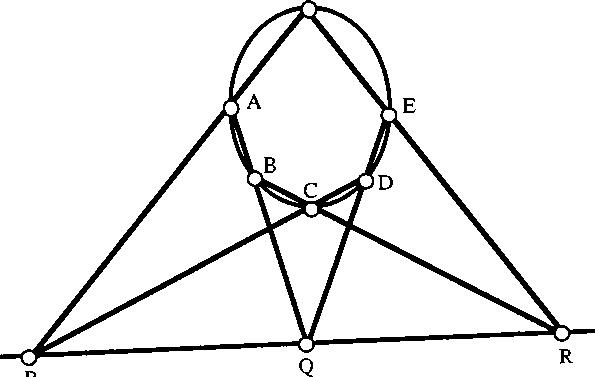
\includegraphics[width=10cm]{37.jpg}\\
			 % \caption{初}
			\end{figure}
		
		
			\textbf{证明} \ 在图中, 考虑两组直线
			\begin{equation*}
				L_{1}:PAF, L_{2}:QDE, L_{3}:RBC	
			\end{equation*}
			和
			\begin{equation*}
				M_{1}:PCD, M_{2}:QAB, M_{3}:REF	
			\end{equation*}
			令$C_{1}=L_{1}+L_{2}+L_{3},C_{2}=M_{1}+M_{2}+M_{3}$, 应用2.7,显然$C_{1}$和$C_{2}$是两条三次曲线且满足
			\begin{equation*}
			C_{1} \cap C_{2}=\{A,B,C,D,E,F,P,Q,R\}
			\end{equation*}
			假如$ PQR $共线, $ L=PQR $; 令$\Gamma$为过$ ABCDE $的圆锥曲线(其存在唯一性由推论1.11给出). 然后, 通过构造,$L+\Gamma$是一条通过8个点$ A,B,C,D,E,P,Q,R $的三次曲线, 则通过(2.7), 它一定通过点$ F $, 即$F \subset L \cup \Gamma$; 根据假设$F \notin L$, 所以$F \in \Gamma$, 故六点共圆锥曲线.
		
		
			反过来, 假设$ ABCDEF $在一个圆锥曲线$\Gamma$上, 令$ L=PQ $,则$L+\Gamma$是一个通过$ A,B,C,D,E,F,P,Q $的三次圆锥曲线,由2.7知,它一定通过$ R $. $ R $不可能在圆锥曲线$\Gamma$上(否则$\Gamma$是一对直线或图中6条线中的一些会重合),所以$R\in L$, 即$ PQR $共线.
	\section{拐点, 标准形式}
		$\mathbb{P}^{2}_{R}$或$\mathbb{P}^{2}_{C}$中有能被写成标准形式
		\begin{equation*}
		C:Y^{2}Z=X^{3}+aXZ^{2}+bZ^{3}
		\end{equation*}
		或仿射形式
		\begin{equation*}
		C:y^{2}=x^{3}+ax+b
		\end{equation*}的曲线
	
		
		现在考虑上述曲线C; 它与无穷远直线$ L:(Z=0) $在何处相交?那很容易,只要把$ Z=0 $代入$F=-Y^{2}Z+X^{3}+aXZ^{2}+bZ^{3}$得到$F|_{L}=X^{3}$; 这意味着$F|_{L}=X^{3}$在$ P(0,1,0) $处有一个三重零点.
		
		为了看看这在几何上代表什么,令$ Y=1 $,得到$ (0,1,0) $附近关于仿射坐标$ (x,z) $的方程:
		\begin{equation*}
		C:z=x^{3}+axz^{2}+bz^{3}
		\end{equation*}
		这个曲线高度近似于$z=x^{3}$:
		
		
		\begin{figure}[h]
		  \centering
		  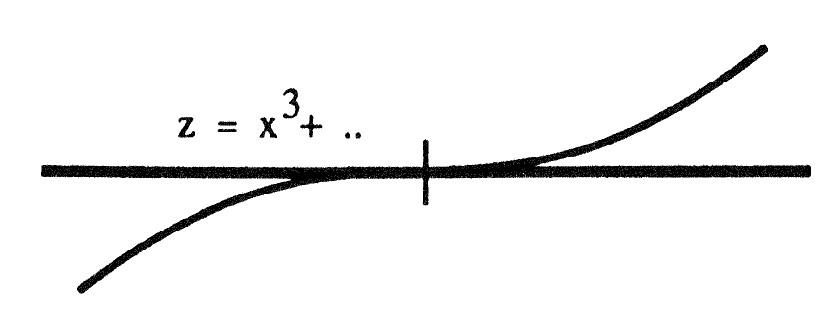
\includegraphics[width=5cm]{38.jpg}\\
		 % \caption{初}
		\end{figure}
	
	
	
		这说明$ C $在$ (0,1,0) $处有一个拐点.
		
		
		更一般地,$ C $上有一个拐点$ P $的定义是存在一条直线$L\subset \mathbb{P}^{2}_{k}$,使$F|_{L}$在$ P $点有一个 重数大于等于3 的零点(见习题2.9;事实上需要$L=T_{P}C(2.8,b)$且重数=3(1.9)), 不难用定义方程的导数和二阶导数来说明这一点, 如果定义方程是$ y=f(x) $, 那么$ P $为拐点的条件是,$\frac{d^{2}f}{dx^{2}(P)}=0$, 这在图中对应一个从凹向下到凹向上变化的曲线. 根据Hessian得知平面曲线是否有拐点有一个标准,见[Fulton,p.116]或\textit{练习7.3},(iii).
		
		
		反过来,如果一条曲线$ C $有拐点,那么它的表达式一定能写成标准形式$C:Y^{2}Z=X^{3}+aXZ^{2}+bZ^{3}$.
	\section{简化的群}
		在标准形式
		$P^{2}_{R}$或$P^{2}_{C}$中有能被写成标准形式
		\begin{equation*}
		C:Y^{2}Z=X^{3}+aXZ^{2}+bZ^{3}
		\end{equation*}
		的曲线上定义群很方便:将点$ O(0,1,0) $作为零元. 在这些条件下,群的建立会很好,有以下几点原因:
		
		(a)$C={O}\cup C_{0}:(y^{2}=x^{3}+ax+b)$, 所以可将曲线$ C $看作一条仿射曲线和无穷远一点O,即群的零元.
		
		(b)过O的直线是(2.8)(i)群的构造的主要部分,由$X=\lambda Z$给出,仿射坐标系中为$x=\lambda$; 这样的直线与C的交点或者是$(\lambda,\pm \sqrt{\lambda^{3}+a\lambda+b})$, 或者是无穷远点$ O $. 因此如果点$ P $的坐标为$ (x,y) $, 则(2.8,i)中构造的$\bar{P}$为$ (x,-y) $, 所以映射$P\mapsto\bar{P}$由 $(x,y)\mapsto(x,-y)$给出.
		
		\begin{figure}[h]
		  \centering
		  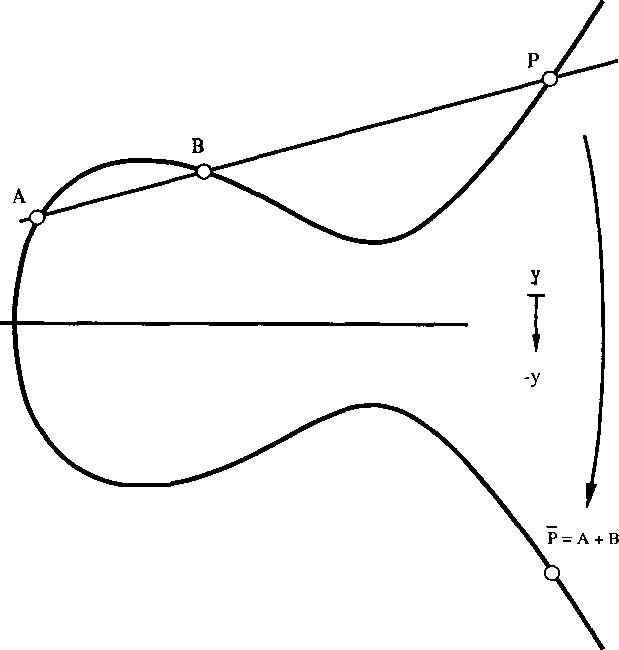
\includegraphics[width=5cm]{39.jpg}\\
		 % \caption{初}
		\end{figure}
	
	
	
		(c)由(2.8,IV),群的逆由$\bar{O}$给出,$\bar{O}$是以O为2重零点的直线L与C的第三个交点;在我们现在的情况下,这条直线是无穷远直线$ L:(Z=0) $且$L\cap C=3O$, 所以$\bar{O}=O$,群的逆简化为$-P=\bar{P}$.
		
		
		\textbf{定理} \ 
		$ C $是由标准形式$C:Y^{2}Z=X^{3}+aXZ^{2}+bZ^{3}$给出的一条三次曲线,那么在$ C $上有唯一的群使得$ O=(0,1,0) $是零元,元素的逆由由 $(x,y)\mapsto(x,-y)$给出, 且对任意的$P,Q,R\in C$,
		\begin{equation*}
			P+Q+R=O \Longleftrightarrow P,Q,R\text{共线}
		\end{equation*}
		
		
		\justifying	
		\textbf{证明} \ 左 $\Rightarrow$ 右 \   $P+Q=-R=\bar{R}$, 所以$ PQ $与$ C $的第三的交点为$ R $,即$ P,Q,R $共线.
		
		右$\Leftarrow$左 \ $P+Q=\bar{R}=-R$, 所以$ P+Q+R=O $.

	\section*{练习2}
		\subsection{在$C:\left(y^{2}=x^{3}+4 x\right)$上建立如(2.13)给出的简化群律.证明:曲线$ C $在$ P = (2,4) $处的切线经过$ (0,0) $,并且$ P $在群中是四阶元.}
			证明:
			
			
			联立方程$
			\left\{
			\begin{aligned}
			y^{2}=x^{3}+4 x \\
			y = 2x\\
			\end{aligned}
			\right.
			$得到方程在$ (0,0) $处有一个根,在$ (2,4) $处有一个二重根.
			
			
			根据习题2.3的结论,显然经过(0,0)和(2,4)的直线是曲线$ C $在(2,4)的切线.
			
			
			设(0,0)为点A,根据(2.13)给出的简化群律,$ P + P =  A$,同时$ A+A = O $,则此时有$ 4P = O $即$ P $是四阶元.
			
		\subsection{曲线$C:\left(y^{2}=x^{3}+ax+b\right) \subset \mathbb{R}^{2}$是非奇异的,找出建立在曲线上的群中所有的二阶元并解释所有二阶元形成的群(这可以分成两种情况),然后几何性地解释如何找出所有的四阶元.}
			
			解:
			
			
			对于方程$ x^{3}+ax+b = 0 $,显然它的解有两种情况:
			
			
			1.有一个实根和两个虚根,设实根为$ x = a $
			
			
			在这种情况下,点$ (a,0) $是唯一的二阶元,此时所有二阶元组成的群是二阶循环群.
			
			
			2.有三个实根,设实根分别为$ x = a $,$ x = b $,$ x = c $
			
			
			在这种情况下,点$ (a,0) $,$ (b,0) $,$ (c,0) $都是二阶元,并且所有二阶元组成的群是克莱因四元群.
			
			
			根据习题2.4的结论,所有四阶元处的切线都经过二阶元,则过二阶元作曲线的切线可找出所有的四阶元.
			
		\subsection{$ x,z $是$ k^{2} $上的一组基底,对$f \in k[x, z]$有}
			\begin{equation*}
			f=a+b x+c z+d x^{2}+e x z+f z^{2}+\ldots
			\end{equation*}
			当$ f $递进地满足下列条件时,写出参数$ a,b,c \ldots $的取值
			\begin{enumerate}[(i)]
				\item $P=(0,0) \in C:(f=0)$;
				\item $ C $在$ P $点处的切线是$ (z = 0) $;
				\item $ P $是$ C $上的拐点并且$ (z = 0) $是切线.
			\end{enumerate}
		
			解:
			\begin{enumerate}[(i)]
				\item 将$P(0,0)$点代入方程,得$ a = 0 $.
				\item 将隐函数$ a+b x+c z+d x^{2}+e x z+f z^{2}+\ldots = 0 $对$ x $求导,得$ b+c z'+2d x+e z+exz'+2f zz'+\ldots = 0 $
				
				
				将$ x = 0,z' = 0 $代入,得$ b = 0 $
				\item 联立方程$
				\left\{
				\begin{aligned}
				f = 0 \\
				z = 0\\
				\end{aligned}
				\right.
				$由(2.12)知方程在(0,0)处有三重及以上重数的根,即$ c = 0,f = 0 $
			\end{enumerate}
		
		
\chapter{仿射簇和希尔伯特零点定理}
	前半部分大多是纯交换代数.在这一章中,环意味着有单位元的交换环.
	\section{命题与定义}
		下面的条件对于环A来说等价.
		
		
		(i)每个理想$I \subset A$是有限生成的.即,任意理想$I \subset A$,存在$f_{1},...,f_{k} \in A$, 使得$I=(f_{1},...,f_{k}).$
		
		
		(ii)每一条A的理想构成的升链
		
		
		\begin{equation*}
			I_{1} \subset ... \subset I_{m} \subset ...
		\end{equation*}
		
		
		会终止,即有$I_{N}=I_{N+1}=...$(升链条件,a.c.c).
		
		(iii)A的非空理想有极大元.
		
		
		满足以上三个条件,A称为诺特环.
		
		
		\textbf{证明}\ $(i) \Rightarrow (ii)$\ 假定$I_{1} \subset ... \subset I_{m} \subset ...$,设$I= \bigcup I_{m}$显然I仍为理想.如果$I=(f_{1},...,f_{})$, 那么任意$f_{i}$都是$I_(m(i))$的元素,所以取$m=max(m(i))$令$I=I_{m}$,升链在此终止.
		
		
		$(ii) \Rightarrow (iii)$\ 由选择公理,显然成立.
		
		
		$(iii) \Rightarrow (i)$\ I为任意理想,$\sum={J \subset I|J是有限生成理想}$.由(iii),$\sum$有极大元,设为$J_{0}$.但是$J_{0}=I$,否则任意$f \in J_{0}$可给出理想$J_{0}+Af$,它是有限生成的但比$J_{0}$大.
		
		
		请证明$\mathbb{Z}$和$ k[X] $是诺特环.
		
	\section{命题}
		(i)A为诺特环,$I \subset A$为理想,那么商环B=A/I为诺特环.
		
		
		(ii)令A为诺特整环,$A \subset K$为分式域,$0 \notin S \subset A$是子集,令
		
		
		\begin{center}
			$B=A[S^{-1}]={a/b \in K|a \in A,且b=1或是S中元素的乘积}$.
		\end{center}
		
		
		证明参考3.4.
		
		
	\section{希尔伯特基定理}
		环A有,
		
		
		\begin{center}
			A是诺特环$\Rightarrow$A[X]是诺特环.
		\end{center}
		
		
		\textbf{证明}\ 令$J \subset A[X]$是任意理想,证明J有限生成.定义首项为n次的J的元素为
		
		
		\begin{center}
			$J_{n}={a\in A|\exists f=aX^{n}+b_{n-1}X^{n-1}+..+b_{0}\in I}$.
		\end{center}
		
		
		那么$J_{n}$是A的理想而且$J_{n} \subset J_{n+1}$.因此,由升链条件,存在N使$J_{N}=J_{N+1}=...$.
		
		
		建立J的生成元集:对于$i \leqslant N$,令$a_{i1},...,a_{im(i)}$为$J_{i}$的生成元,在$J_{i}$的定义里,对每个$a_{ik}$,令$f_{ik}=a_{ik}X^{i}+...\in J$为i次首项为$a_{ik}$的元素.
		
		
		下证集
		
		
		\begin{center}
			${f_{ik}|i=0,...,N,k=1,...,m(i)}$
		\end{center}
		
		
		生成J:对给定的$g\in J$,假定deg g = m.那么g的首项为$bX_{m}$,$b\in J_{m}$.有$b=\sum c_{m'k}a_{m'k}(这里m'=m若m\leqslant N,否则m'=N)$.然后考虑$g_{1}=g-X^{(m=m')} \sum c_{m'k}f_{m'k}$:通过构造可使m次数为0,所以$deg g_{1} \leqslant deg g-1$;最终可写出g由$f_{ik}$组合而成的形式,所以生成J.
		
		
		\textbf{推论}\ 若k为域,那么有限生成k代数为诺特环.
		
		
		有限生成k代数是一个形如$A=k[a_{1},...,a_{n}]$的环,所以A是由k与$a_{1},...,a_{n}$有限生成的环.很明显,每个这样的环都同构于一个多项式环的商环,$A \backsimeq k[a_{1},...,a_{n}]/I$.域是诺特环,由(3.3),$k[a_{1},...,a_{n}]$是诺特环,最后由(3.2)(i)商环也是诺特环.
		
		
	\section{对应V}
		k是任意域,$A=k[a_{1},...,a_{n}]$.记$\mathbb{A}^{n}_{k}=k_{n}$为k上n维仿射平面.$k(a_{1},...,a_{n})\in A$点$P=(a_{1},...,a_{n}) \in \mathbb{A}^{n}_{k}=k_{n}$,$f(a_{1},...,a_{n}) \in k$.定义对应V
		
		
		\begin{center}
			${理想J \subset A} \longrightarrow {子集X \in \mathbb{A}^{n}_{k}}$
			
			
			$J \longmapsto V(J)={P \in \mathbb{A}^{n}_{k}|f(P)=0对任意f \in J}$
		\end{center}
		
		
		\textbf{定义}\ 子集$X \subset \mathbb{A}^{n}_{k}$是代数集如果X=V(I)对某些I成立.由3.3,I为有限生成的.如果$I=(f_{1},...,f_{r})$那么显然
		
		
		\begin{center}
			$V{I}={P \in \mathbb{A}^{n}_{k}|f_{i}(P)=0,i=1,..,r}$
		\end{center}
		
		
		所以代数集是满足一个多项式方程的有限点的轨迹.
		
		
		若I=(f)是主理想,那么通常把V(I)写成V(f).
		
		
	\section{命题与定义}
		对应V满足:
		
		
		$(i)V(0)=\mathbb{A}^{n}_{k};V(A)=\phi$;
		
		
		$(ii)I \subset J \Rightarrow V(I)\supset V(J)$;
		
		
		$(iii)V(I_{1} \bigcap I_{2}) = V(I_{1}) \bigcup (I_{2})$;
		
		
		$(iv)V(\sum _{\lambda \in \Lambda}I_{\lambda})=\bigcap _{\lambda \in \Lambda}V(I_{\lambda})$
		
		
		因此$\mathbb{A}^{n}_{k}$的代数集构成了$\mathbb{A}^{n}_{k}$上拓扑的闭集,Zariski拓扑.
		
		
		只给出(iii)的$\subset$的证明.设$P\notin V(I_{1}) \bigcup (I_{2})$,有$f\in I_{1},g\in I_{2}$使得$f(P) \ne 0,g(P) \ne 0$.所以$fg\in I_{1} \bigcap I_{2}$,但$fg(P) \ne 0$,因此$P\notin V(I_{1} \bigcap I_{2})$.
		
		
	\section{对应I}
		V的某种逆,有对应I
		
		
		\begin{center}
			${理想J\subset A} \longleftarrow {子集X \subset \mathbb{A}^{n}_{k}}$
			
			
			$I(X)={f \in A|f(P)=0,任意P\in X} \gets X$
		\end{center}
		
		
		这意味着I把X映成在X上为0的函数.
		
		
		\textbf{命题}\ (a)$X\subset Y \Rightarrow I(X) \supset I(Y)$;
		
		
		(b)对任意子集$X \subset \mathbb{A}^{n}_{k}$,有$X \subset V(I(X))$当且仅当X为代数集;
		
		
		(c)对$J \subset A$,有$J \subset I(V(J))$;为严格包含.
		
		
		$\textbf{证明}$\ (a)显然.(b)与(c)的包含为同义反复的:I(X)被定义为在X上所有点为0的函数集,那么对于X中一点,所有I(X)中函数在其上为0.
		
		
		(b)中剩下的部分很简单:若X=V(I(X))那么V是代数集,因为它为形式V(某理想).相反地,如果$X=V(I_{0})$是代数集,那么I(X)至少包含$I_{0}$,故$V(I(X))\subset V(I_{0})=X$.
		
		
		有两种可能使(c)中的包含为严格的.
		
		
		$\textbf{例1}$\ 假设k不是代数闭的,令$f\in k[X]$为一个非常数多项式,且在k中没有根.考虑理想$J=(f)\subset k[X]$.那么$J\ne k[X]$,因为$1\notin J$.但
		
		
		\begin{center}
			$V(J)={P\in \mathbb{A}^{1}_{k}|f(P)=0=\phi}$
		\end{center}
		
		
		因此I(V(J))=k[X].
		
		
		所以如果域不是代数闭的,可能无法有足够的零点.一个相似的例子:在$\mathbb{R}^{2}$,多项式$X^{2}+Y^{2}$定义了单点$P=(0,0)$,故$V(X^{2}+Y^{2})={P}$.但是除此之外还有很多在{P}为0的多项式,而且事实上I(P)=(X,Y).
		
		
		$\textbf{例2}$\ 对任何$f\in k[X_{1},...X^{2}]$且$a\geqslant 2$,$f^{a}$定义了与f相同的轨迹,$f^{a}(P)=0\iff f(P)=0$.所以$V(f^{a})=V(f)$,且$f\in I(V(f^{a}))$,但是通常$f\notin (f^{a})$.在例1中,讨论的是$X^{2}=0$定义的两条直线,它只能意味着(X=0)平方了,但事实并非如此.
		
		
	\section{不可约代数集}
		一个代数集$X\subset \mathbb{A}^{n}_{k}$是不可约的,如果不存在分解
		
		
		\begin{center}
			$X=X_{1}\cup X_{2}当X_{1},X_{2}\varsubsetneq X$
		\end{center}
		
		
		比如,代数集$V(xy)\subset \mathbb{A}^{n}_{k}$是由两坐标轴组成的轨迹,显然是V(x)与V(y)的组合,所以是可约的.
		
		
		$\textbf{命题}$\ (a)令$X\subset \mathbb{A}^{n}_{k}$是代数集且I(X)是对应的理想.那么
		
		
		\begin{center}
			X是不可约的 $\iff$ I(X)是素理想.
		\end{center}
		
		
		(b)任何代数集X有唯一分解
		
		
		\begin{center}
			$X=X_{1}\cup...\cup X_{r}$ $\rightline{(*)}$
		\end{center}
		
		
		$X_{i}$不可约且$X_{i}\nsubseteq X_{j}$当$i\ne j$.
		
		
		$\text{证明}$\ (a)要证X是不可约的$\iff$I(X)不是素的.
		
		
		$(\Rightarrow)$设$X=X_{1} \cup X_{2}$,$X_{1}\nsubseteq X$ 意味着有$f_{1}\in I(X_{1})/X$,相似地$X_{2}\nsubseteq X$ 意味着有$f_{2}\in I(X_{2})/X$.$f_{1}f_{2}$在X的所有点上为0,故$f_{1}f_{2}\in I(X)$.则I(X)不是素的.
		
		
		$(\Leftarrow)$设I(X)不是素的,有$f_{1},f_{2}\notin I(X)$使$f_{1}f_{2}\in I(X)$.让$I_{1}=(I(X),f_{1})$且$V(I_{1})=X_{1}$,那么X的真子集$X_{1}$为代数集.同理,得到$X_{2}$. 由$X\subset X_{1}\cup x_{2}$,对任意$P\in X$,$f_{1}f_{2}(P)=0$意味着$f_{1}(P)=0$,$f_{2}(P)=0$.
		
		
		(b)$\mathbb{A}^{n}_{k}$中代数集构成链
		
		
		\begin{center}
			$X_{1}\supset X_{2}\supset ... \supset X_{n} \supset...$
		\end{center}
		
		
		最终终止.这是因为
		
		
		\begin{center}
			$I(X_{1})\subset I(X_{2})\subset ... \subset I(X_{n}) \subset...$
		\end{center}
		
		
		是A的理想构成的升链.正如在3.1中,
		
		
		\begin{center}
			$\mathbb{A}^{n}_{k}$上代数集的任何非空$\sum$有极小元.$\rightline{(!)}$
		\end{center}
		
		
		令$\sum$为$\mathbb{A}^{n}_{k}$的代数子集,它没有分解(*).若$\sum=0$那么(b)成立,否则,由(!),必有极小元$X\in \sum$,这样有:若X不可约,那么$X\notin \sum$,矛盾;若X可约,那么$X= X_{1}\cup x_{2}$,$X_{1},X_{2}$为X的真子集.又X为极小元,$X_{1},X_{2}\nsubseteq \sum$.所以$X_{1},X_{2}$各有分解(*),把它们合并有(*)的分解,故$X\notin \sum$.所以$\sum =0$.(b)得证.
	\section{断言}
		让k为有限域,$A=k[a_{1},...,a_{n}]$是有限生成k代数.那么
		
		
		\begin{center}
			A是数域 $\Rightarrow$ A在k上是代数的
		\end{center}
		
		
		粗略证明:若$t\in A$是k上超越元,那么k[t]是多项式环,有无限多个素元.因此扩张$k\subset k(t)$不是有限生成的k代数:有限多个元素$p_{i}/q_{i}\in k(t)$只能有有限多个素的生成元.
	\section{希尔伯特零点定理}
		假设$ k $是一个代数闭域.
		\begin{enumerate}[(a)]
			\item 多项式环$A=k \left[X_{1}, \dots X_{n}\right]$中的极大理想总是有着$m_{P}=\left(X_{1}-a_{1}, \ldots X_{n}-a_{n}\right)$的形式,其中$P=\left(a_{1}, \ldots a_{n}\right) \in \mathbb{A}^{n}_{k}$;也就是说,极大理想是在$ P $处取0值的所有函数的理想$ I(P) $.
			\item 如果$J \subset A$是一个理想,$J \neq(1)$,则$V (J ) \neq \varnothing$.
			\item 对于任意$J \subset A$,$ I(V(J)) = rad J$
		\end{enumerate}
		定理的必要条件是$ (b) $,即如果一个理想$ J $不是整个环$ k \left[X_{1}, \dots X_{n}\right] $,则理想中的多项式就会在$ \mathbb{A}^{n}_{k} $上有零点.注意,如果$ k $不是代数闭域,那么$   (b) $就是完全错误的,因为如果$f \in k [ X ]$是一个非常数多项式,那么$ f $就不能作为一个理想来生成整个$ k [ X ] $,但是可能有$ V(f) = \varnothing \subset \mathbb{A}^{1}_{k} $.
		
		
		\textbf{推论}\ 对应关系$ V $和$ I $
		
		
		\centerline{$\{\text { 理想 } I \subset A \}\quad{\stackrel{ V , I }{\longleftrightarrow}} \quad\left\{\text {子集} X \subset A ^{ n } k \right\}$}
		
		
		导出双射$ \qquad\qquad\qquad\qquad\quad\cup\qquad\qquad\qquad\qquad\qquad\cup $
		

		\centerline{\{根理想\} \qquad $\longleftrightarrow$ \qquad \{代数子集\}}
		
		
		以及$ \qquad\qquad\qquad\qquad\qquad\quad\cup\qquad\qquad\qquad\qquad\qquad\cup $
		
		
		\centerline{\qquad\quad \{素理想\} \qquad $\longleftrightarrow$ \qquad \{不可约代数子集\}}
		
		
		上述双射成立时因为由(3.6, b)对任意代数集$ X $有$ V(I(X))  = X$,而由(3.10, c)对任意根理想$ J $有$ I(V(J))  = J$.
		
		
		\textbf{零点定理的证明(假设3.8成立)}
		
		
		$ (a) $\ 设$m \subset k \left[ X _{1}, \ldots X _{ n }\right]$是一个极大理想,取$K = k \left[ X _{1}, \ldots X _{ n }\right] / m$,则有$ \varphi $是两个自然映射的合成$ \varphi : k \to k \left[ X _{1}, \ldots X _{ n }\right] \to K$.则$ K $是一个域(因为$ m $是极大的),而作为k-代数$ K $是有限生成的(因为$ K $由$ X_{i} $的象生成).所以由(3.8),$ \varphi : k \to K $是一个代数的域扩张.但是$ k $是代数闭域,所以$ \varphi $是一个同构.
		
		
		现在,对每一个$ i $,$X _{ i } \in k \left[ X _{1}, \ldots X _{ n }\right]$映到一些元素$ b_{i} \in K$,所以取$a _{ i =} \varphi^{-1}\left(b _{ i }\right)$则有$X _{ i }- a _{ i } \in \operatorname{Ker}\left\{ k \left[ X _{1}, \ldots X _{ n }\right] \rightarrow K \right\}= m .$因此这里存在$a _{1}, \ldots a _{ n } \in k$使得$\left(X _{1}- a _{1}, \ldots X _{ n }- a _{ n }\right) \subset m .$另一方面,左侧显然是一个极大理想,因此$\left(X _{1}- a _{1}, \ldots X _{ N }- a _{ n }\right)= m .$则$ (a) $得证.
		
		
		$ (a)  \Rightarrow (b) $\ 这一部分证明是简单的.如果$J \neq A = k \left[ X _{1}, \ldots X _{ n }\right]$,那么对$ A $一定存在一个极大理想$m$使得 $J \subset m$ ($ m $的存在性是显然的,可以利用升链条件).由$ (a) $,$ m $具有形式$m =\left(X _{1}- a _{1}, \ldots X _{ n }- a _{ n }\right)$,则 $J \subset m$ 意味着对于任意 $f \in J$有$f (P )=0$ ,其中$P =\left(a _{1}, \ldots a _{ n }\right) .$因此$P \in V (J )$.
		
		
		$ (b)  \Rightarrow (c) $\ 这一部分需要一个小技巧.设$J \subset k \left[ X _{1}, \ldots X _{ n }\right]$是任意理想,而$f \in k \left[ X _{1}, \ldots X _{ n }\right]$.引入另外一个变量$ Y $,考虑由$ J $和$ fY - 1 $生成的新理想
		\begin{equation*}
		J _{1}=(J , f Y -1) \subset k \left[ X _{1}, \ldots X _{ n }, Y \right]
		\end{equation*}
		粗略地说,$ V(J_{1}) $是一个包含$ P \subset V(J) $的簇,因此$ f(P) \neq 0 $.更准确地说,一点$Q \in V\left(J_{1}\right) \subset \mathbb{A}^{n+1}_{k}$是一个$ n +1 $元$Q =\left(a _{1}, \ldots a _{ n },b \right)$使得
		\begin{equation*}
		\text {对所有} g \in J \text{有}g\left(a_{1}, \dots a_{n}\right)=0 , \text { 即} P=\left(a_{1}, \dots a_{n}\right) \in V(J)
		\end{equation*}
		以及
		\begin{equation*}
		f(P) \cdot b=1, \text {即} f(P) \neq 0 \text { 且 } b=f(P)^{-1}.
		\end{equation*}
		
		
		现在假设对所有$ P \subset V(J) $有$ f(P) = 0 $,则显然由上文可得$ V(J_{1}) = \varnothing $.因此由$ (b) $可推出$ 1 \in J_{1}$,即存在表示
		\begin{equation*}
		\left.1=\sum g_{i} f_{i}+g_{0}(f Y-1) \in k | X_{1}, \ldots X_{n}, Y\right]
		\end{equation*}
		其中$ f_{i} \in J $而$ g_{0},g{i} \in k \left[ X _{1}, \ldots X _{ n }, Y \right] $.
		
		
		考虑为什么上式中$ Y $在右侧:除了显式地表示,$ Y $还存在在每一个$ g_{i} $中,假设$ Y^{N} $是$ Y $在$ g_{0},g{i} $中存在的最高阶.如果将两边同乘$ f^{N} $,就有关系
		\begin{equation*}
		f ^{ N }=\sum G _{ i }\left(X _{1}, \ldots X _{ n }, f Y \right) f _{ i }+ G _{0}\left(X _{1}, \ldots X _{ n }, fY \right)(fY -1)
		\end{equation*}
		其中$ G_{i} $是$ f^{N}g_{i} $用$ X _{1}, \ldots X _{ n } $和$ (fY) $的多项式形式写出来的.
		
		
		上式是仅关于$ k \left[ X _{1}, \ldots X _{ n }, Y \right] $的多项式的等式,因此可以两边同模$ (fY -1) $得到
		\begin{equation*}
		f ^{ N }=\sum h _{ i }\left(X _{1}, \ldots X _{ n }\right) f _{ i } \in k \left[ X_{1}, \ldots X _{ n }, Y \right] /(f Y -1)
		\end{equation*}
		等式两边都是$ k \left[ X _{1}, \ldots X _{ n }\right] $中的元素.因此自然的同态$ k \left[ X _{1}, \ldots X _{ n }\right] \hookrightarrow k \left[ X _{1}, \ldots X _{ n }, Y \right] /(f Y -1)$是一个内射(这是$ k \left[ X _{1}, \ldots X _{ n }\right] $到$ k \left[ X _{1}, \ldots X _{ n }\right][f^{-1}] $的一个自然嵌入,就像子环和它的分式域一样),它遵循
		\begin{equation*}
		f ^{ N }=\sum h _{ i }\left(X _{1}, \ldots X _{ n }\right) f _{ i } \in k \left[ X _{1}, \ldots X _{ n }\right]
		\end{equation*}
		即对任意$ N $有$ f^{N} \in J $.则证毕.
		
		
	\section{一些实例}
		\textbf{(a)超平面}
		
		
		关于簇的一个最简单实例是超平面$V (f ):(f =0) \subset \mathbb{A} ^{ n } k$.如果$ k $是代数闭域,那么在不可约元$f \in k \left[ X _{1}, \dots X _{ n }\right]$和不可约超平面上就有一个自然的对应关系:由零点定理,两个互质的不可约多项式$ f_{1},f_{2} $定义了两个不同的超平面$ V(f_{1}),V(f_{2}) $.这并不总是显然的(例如,在$ \mathbb{R} $上就不成立),尽管这不用零点定理而用消去定理(19世纪提出的一个更加显式的方法)就能证明,即\textit{练习3.13}.
		
		
		\textbf{(b)}
		
		
		除了超平面外,绝大多数的簇都是由很多等式来定义的.反直觉地,这通常都是因为理想$ I(X) $有多个生成元,即多于$ X $的共同维数的生成元.例如,对于$C \subset \mathbb{A} ^{3} k$,$ I(C) $需要三个生成元,现在假设$ k $是一个无限域.
		
		
		先考虑,$J =\left(uw - v ^{2}, u ^{3}- vw \right)$.其中$ J$不是素的,因为
		\begin{equation*}
		 J \ni w \left(uw - v ^{2}\right)- v \left(u ^{3}- v w \right)= u \left(w ^{2}- u ^{2} v \right)
		\end{equation*}
		 而$ u , w ^{2}- u ^{2} v \notin J $.因此
		 \begin{equation*}
		 	V (J )= V (J , u ) \cup V \left(J , w ^{2}- u ^{2} v \right)
		 \end{equation*}
		 显然,$ V (J , u ) $是直线$ (u = v =0) $.同时,另外一部分$  C = V \left(J , w ^{2}- u ^{2} v \right)$是一个不可约曲线,而$ C $由三部分给出:
		 \begin{equation*}
		 	uw = v ^{2}, u ^{3}= vw , w ^{2}= u ^{2} v
		 \end{equation*}
		
		
		现在证明$C \subset \mathbb{A} ^{3}$是映射$\varphi: A ^{1} \rightarrow C \subset A ^{3}$在$t \mapsto t^{3}, t^{4}, t^{5}:$下的象:如果$u \neq 0$ 则 $v, w \neq 0 .$取$t=v / u,$ 则$t=w / v /$ 且 $t ^{2}=(v / u )(w / v )= w / u .$因此$v = w ^{2} / u ^{2}= t ^{4}, u = v /(v / u )= t ^{4} / t = t ^{3} /$ 并且
		$w = tv = t ^{5},$ 则 $C$ 是不可约的, 因此如果$C = X _{1} \cup X _{2}, X _{ i } \subset C ,$ 且 $f _{ i }(u , y , w ) \in I \left(X _{ i }\right),$则对于所有 $t ,$ 至少有一个 $f _{ i }\left(t ^{3}, t ^{4}, t ^{5}\right)$取到0值. 因为一个非零多项式至多有有限个零点, $f_{1}, f_{2}$中的一个必须为0,所以$f _{ i } \in I (C )$.
		
		
		这个实例是一个不错的单项式的例子,通常情况下是很难找到一个簇的不可约部分的,更别提证明它不可约了.一个同样的例子为\textit{练习 3.11}
		
		
	\section{有限代数}
		现在开始证明$ (3.8) $.设$A \subset B$都是环.通常来说,如果存在有限个元素$b_{1}, \dots b_{n}$使得$B=A\left[b_{1}, \ldots b_{n}\right],$则$ B $被称作在$ A $上的有限扩张(或$ A- $代数),因此$ B$由$ A $和$b_{1}, \ldots b_{n}$生成.
		
		
		与下述定义做对比:如果存在有限个元素$b_{1}, \dots b_{n}$使得$B=A b_{1}+. . A b_{n},$则$ B $被称作有限$ A- $代数,即,$ B $作为$ A- $模是有限生成的.
		
		
		两个定义最大的不同是一个是作为环(即允许对$ b_{i} $的任意多项式表达),一个是作为模(只允许线性表达).例如,$ k[X] $是一个有限生成$ k- $代数(仅由一个元素$ X $生成),但这不是一个有限$ k- $代数(因为作为$ k- $向量空间它是无限维的).
		
		
		\textbf{命提}\  (i)设 $A \subset B \subset C$都是环: 则
		
		\begin{equation*}
		\begin{split}
		B\text{是} A -\text{代数且}&C \text{是有限} B -\text{代数}\\
		\Rightarrow &C \text {是有限 }A -\text{代数}
		\end{split}
		\end{equation*}
		
		
		(ii) 如果$A \subset B$是一个有限$ A $-代数且 $x \in B$则$x$满足一个在$A$上的首一多项式,即存在关系
		\begin{equation*}
		x^{n}+a_{n-1} x^{n-1}+. . a_{0}=0 \text {其中}a_{i} \in A
		\end{equation*}
		(注意其中首项系数是1).
		
		
		(iii) 反过来,如果$x$满足一个在$A$上的首一多项式,则$B=A[x]$ 是一个有限$ A- $代数.
		
		
		\textbf{证明}\  (i)和(iii)简单的(仿照域扩张的相似结论). 对于(ii),可以使用一个不太显然的行列式技巧:假设$B =\sum A b _{ i } ;$ 则对于任意$i ,  x b_{ i } \in B ,$ 所以有常数$a_ij \in A$使得
		\begin{equation*}
		x b_{i}=\sum_{j} a_{i j} b_{j}
		\end{equation*}
		
		
		也可以写作
		\begin{equation*}
		\sum_{j}\left(x \delta_{i j}-a_{i j}\right) b_{j}=0
		\end{equation*}
		其中$\delta_{ ij }$是单位矩阵.则设$M$是矩阵:
		
		\begin{equation*}
		M _{ i j }=\left(x \delta_{ i j }- a _{ i j }\right)
		\end{equation*}
		
		然后取$\Delta=\operatorname{det} M .$ 然后由标准线性代数, (将$b$写作列向量和项$\left(b_{1}, \dots b_{n}\right)$ 以及$M$的伴随矩阵 $M^adj$).
		\begin{equation*}
		Mb =0, \quad \text { 因此 } \quad 0=\left(M ^{ adj }\right) Mb =\Delta b
		\end{equation*}
		则对所有$ i $有$\Delta b_{i}=0$. 但是, $1_{B} \in B$是关于 $b _{ i }$的线性组合,因此 $\Delta=\Delta \cdot 1 B =0,$最后则得到关系: $\operatorname{det}\left(x \delta_{ ij }- a _{ ij }\right)=0 .$ 则显然有对$x$的首一多项式,而系数则来自$ A $.
		
		
	\section{诺特正规化}
		\textbf{诺特正规化引理}\ 设$k$ 是一个无限域, 同时$A=k\left[a_{1}, \ldots a_{n}\right]$是一个有限生成的$k$ -代数. 则存在$m \leq n$和$y_{1}, . . y_{m} \subset A$使得
		\begin{enumerate}[(i)]
			\item  $y _{1} \ldots y _{ m }$ 在$k$上代数独立;
			\item $A$是有限$k \left[ y _{1}, \dots y _{ m }\right]$ -代数.
		\end{enumerate}
		
		
		((i)意味着对$y_{i}$的线性组合,当且仅当系数全为0时才取到0值; 代数地来讲,就是自然的映射$k \left[ Y _{1}, \ldots Y _{ m }\right] \rightarrow k \left[ y _{1}, \ldots y _{ m }\right] \subset A$是单射.
		
		可以断言,环的扩张可以通过首先引入代数独立的元素,然后“进行代数扩张”来建立.但是,(ii)远比此精确得多,因为它说$ A $中的每个元素不仅是在$ k \left [y _ {1},\ldots y _ {m} \right]$上代数的,还满足在其上的首一多项式.
		
		
		
		\textbf{证明}\ 取$ I $是自然满射的核
		\begin{equation*}
		I =\operatorname{ker}\left\{ k \left[ X _{1}, \ldots X _{ n }\right] \rightarrow k \left[ a _{1}, \ldots, a _{n}\right]= A \right\}
		\end{equation*}
		假设$0 \neq f \in I ;$ 证明的思路是将$X _{1} \ldots X _{ n -1}$ 替换为确定的$X _{1}^{\prime} \ldots X _{ n -1}^{\prime}$使得$f$对于$a _{ n }$在$A ^{\prime}= k \left[ a _{1}^{\prime}, \ldots a ^{\prime} n -1\right]$上是一个首一多项式.
		
		
		
		所以记
		\begin{equation*}
		\begin{array}{c}
		{ a _{1}^{\prime}= a _{1}- c _{1} a _{ n }} \\
		{\cdots} \\
		{ a _{ n -1}^{\prime}= a _{ n -1}- a _{ n -1} a _{ n }}
		\end{array}
		\end{equation*}
		(其中$\alpha_{i}$是$k$ 中的元素).之后有
		\begin{equation*}
		\left.0= f \left(a ^{\prime} 1+\alpha_{1} a _{ n }, \ldots\right) a _{ n -1}^{\prime}+\alpha_{ n -1} a _{ n }, a _{ n }\right)
		\end{equation*}
		
		
		\textbf{断言}\ 选择合适的$\alpha_{1}, \dots \alpha_{n-1} \in k,$则多项式
		\begin{equation*}
		f \left(X _{1}^{\prime}+\alpha_{1} X _{ n , w }, X _{ n -1}^{*}+\alpha_{ n -1} X _{ n }, X _{ n }\right)
		\end{equation*}
		是关于$X _{ n }$的首一多项式.
		
		
		利用上述断言,可以通过归纳法证明该引理:当$ n = 1 $时是显然的;当$ n = n $时,若$I=0$,则显然, 因为$a_{1}, \dots a_{n}$是代数独立的.其他情况下, 取$0 \neq f \in I,$和 $ n = n-1 $时的$\alpha_{1}, \ldots \alpha_{n-1}$;则$f$给出了一个满足$ a_{n} $的首一多项式,其中系数来自$A ^{\prime}= k \left[ a _{1}^{\prime}, \ldots a ^{\prime} n -1\right] \subset A .$ 由归纳假设,存在$y_{1}, \dots y_{m} \in A^{\prime}$使得
		
		\begin{enumerate}[(1)]
			\item $y _{1} \ldots y _{ m }$在$k$上时代数独立的;
			\item $A^{\prime}$ 是有限$k \left[y_{1}, \dots \text { y } m \right]$ -代数. 
		\end{enumerate}
		
		
		则$A = A ^{\prime}\left[ a _{ n }\right]$在$A ^{\prime}$上是有限扩张(由$ (3.12.iii) $),因此由$(3.12, i )$, $ A $在$k \left[ y _{1}, \ldots y _{ m }\right]$上是有限扩张,证毕.
		
		
		
		最后剩下来的是断言的证明. 取$d =\operatorname{deg} f ,$并设
		\begin{equation*}
		f = F _{ U }+ G
		\end{equation*}
		其中$F _{ d }$是$d$次齐次多项式, 另外$\operatorname{deg} G \leq d -1 .$ 则
		\begin{equation*}
		\begin{split}
		&f\left(X_{1}, \dots X_{n-1}, X_{n}\right)=f\left(X_{1}^{\prime}+\alpha_{1} X_{n, },\ldots, X_{n-1}^{\prime}+\alpha_{n-1} X_{n}, X_{n}\right)\\
		=&F _{ d }\left(\alpha_{1}, \ldots \alpha_{n-1}, 1\right) \cdot X _{ n }^{d} +\left(\text {对} X _{ n } \text {的阶数} \leq d -1\text{的部分}\right)
		\end{split}
		\end{equation*}
		
		根据假设有$F _{ d }\left(\alpha_{1}, \ldots \alpha_{ n -1}, 1\right) \neq 0 .$ 因为$F _{ d }$是非零多项式, 这就不难验证这是 $\alpha_{1}, \ldots \alpha_{n-1}$在几乎所有取值的情况 (进一步的证明在\textit{练习3.13}).则证毕.
		
		
		
	\section{注}
		(I)事实上,(3.13)的证明表示可以选择足够好的$y_{1} \ldots y_{m}$使得是对$a_{1}, \dots a_{n}$的 $m$一般线性形式. 为了理解$(3.13),$ 记$I = \ker \left\{ k \left[ X _{1}, \ldots X _{ n }\right] \rightarrow k \left[ a _{1}, \ldots a _{ n }\right]= A \right\},$并且假设$ I $是素的. 考虑$V = V (I ) \subset \mathbb{A} ^{ n } k ;$ 并设$\pi: \mathbb{A} ^{ n } k \rightarrow \mathbb{A} ^{ m } k$是由$y_{1}, \dots y_{m},$ 和 $p=\pi | v: V \rightarrow \mathbb{A} m_{k}$定义的线性投影. 这就可以看出(3.13)的结论(i) 和(ii)  意味着在每一个$P \in \mathbb{A} ^{ m } k $ 上, $ p ^{-1}(P )$是一个无限非空集 (即\textit{练习3.16}). 
		
		
		(II)(3.13)的证明也有一个简单的几何解释:从$ n $个变量$X _{1}, \ldots X _{ n }$中选取$n -1$ 个线性形式对应于构造一个线性投影 $\pi: \mathbb{A} ^{n}_{k} \rightarrow \mathbb{A} ^{n-1}_{k} ;$ $\pi$中的线条就构成了一个 $(n-1)-$维平行线簇. 选取多项式$f \in I ,$就不难看出当且仅当没有一个平行线的渐近线是$ (f = 0) $则$f$给出了一个关于最后的$X_{n}$的首一多项式;在射影几何中,这意味着无穷远点$\left(0, \alpha_{1}, \dots \alpha_{n-1}, 1\right) \in \mathbb{P} ^{n-1}_{k}$代表着平行投影不属于$ (f = 0) $上的射影闭集.
		
		
		(III)上面关于(3.13)的证明在有限域上并不成立(即\textit{练习3.14 }).但是定理本身是不需要任何关于$ k $的条件的.
		
		
	\section{(3.8)的证明}
		$A=k\left[a_{1}, \ldots a_{n}\right]$是一个有限生成的$k$ -代数.假设$y _{1}, \ldots y _{ m } \in A$ 满足$(3.13)$中的条件,并记$B = k \left[ y _{1}, y _{ m }\right] .$ 则$A$是一个有限$B$ -代数,已知$A$是一个域.若$B$是一个域, 那么就有 $m =0,$ 使得$A$是一个有限$k$ -代数,即,$k $的一个有限域扩张,(3.8) 则得证. 因此仅需证:
		
		\textbf{引理}\ 若$A$是一个域, 同时$B \subset A$ 是一个子环使得$A$是一个有限$B$ -代数, 那么$B$ 就是一个域.
		
		\textbf{证明}\ 对任意$0 \neq b \in B$,它的逆$b ^{-1} \in A$ 在$ A $中. 则由 (3.12的 ii). $b ^{-1}$ 对于$B$有一个首一多项式,即存在关系
		\begin{equation*}
		b ^{- n }+ a _{ n -1} b ^{-(n -1)}+\ldots a _{1} b ^{-1}+ a _{0}=0, \quad \text { 其中} a _{ i } \in B
		\end{equation*}
		两边同乘$b ^{ n -1}$
		\begin{equation*}
		b ^{-1}=-\left(a _{ n -1}+ a _{ n -2} b +\ldots a _{0} b ^{ n -1}\right) \in B
		\end{equation*}
		因此$B$ 是一个域.这就证明了(3.8)并完成了零点定理的所有证明.
		
		
	\section{}
		\textit{为了让上述证明在特征$ p $的域上是成立的,在这里做一些调整使其更普适.这一段会用到伽罗瓦理论的分离性内容,如果对此毫无头绪可以略过本段.}
		
		\textbf{附录}\ 在 $(3.13)$的条件下,如果更进一步设$k$是代数闭的, 且$A$ 是一个整环并且有分式域$K$,那么就可以像上面一样挑出$y_{1}, \ldots y_{m} \in A$满足(i)和(ii),并且另外满足条件(iii) $\quad k \left(y _{1}, \dots y _{ m }\right) \subset K$是一个可分扩张.
		
		
		\textbf{证明}\ 如果$k$是特征$0$的,那么所有域扩张都是可分扩张;假设$k$是特征$ p $的.因为$A$ 是一个整环,$ I $是素的; 因此如果 $I \neq 0,$那么它就包含一个不可约元$ f $. 现在对任意$ i $这里有两种情况:要么$t$ 在$X _{ i }$上是可分的,要么有$f \in k \left[ X _{1}, \ldots X _{ i }^{ P }, \ldots X _{ n }\right]$.
		
		
		\textbf{断言}\ 如果$ f $在每一个$ X_{i} $上都不可分,那么$ f = g^{P} $,与$ f $的不可分性冲突.
		
		假设$f$具有形式:
		\begin{equation*}
		f = F \left(X _{1}^{ D }, \ldots X _{ n }^{ D }\right), \text {其中} F \subset k \left[ X _{1}, \ldots X _{ n }\right]
		\end{equation*}
		设$g \in k \left[ X _{1}, \ldots X _{ n }\right]$是取系数为$F$的第$ p $个根所做成的多项式,然后重复使用在特征$ p $上的恒等式 $(a+b) P=a P+b P$, 这就容易看出$ f = g^{P} $.
		
		因此任意不可约的$f$至少在一个$X_{i}$中是可分的,不妨设为 $X _{ n } .$然后就像上文一样,有
		\begin{equation*}
		f \left(X _{1}^{\prime}+\alpha_{1} X _{ n }, \ldots X _{ n -1}^{\prime}+\alpha_{ n -1} X _{ n }, X _{ n }\right)
		\end{equation*}
		这是一个首一多项式,这个可分关系是在$A ^{\prime}= k \left[ a _{1}^{\prime},\ldots a _{ n -1}^{\prime}\right]$上对$ a_{n} $成立的. 最后,由相同的归纳可以证明,可分域扩张的合成依然是可分的.则得证.
		
		
	\section{降至超平面}
		在伽罗瓦理论中,有以下结论
		
		\textbf{本原元定理}. 设$K$是一个无限域, 且 $K \subset L$是一个有限可分的域扩张; 那么就存在$x \in L$使得 $L=K(x) .$进一步,如果$ L $是在 $K$上由元素 $z_{1}, \ldots z_{k }  $生成的,那么$x$可以通过$ z_{i} $的线性组合即$\sum_{i} \alpha_{i} z_{i}$表出.
		
		
		(下列是来自伽罗瓦理论的基本定理: 如果$K \subset M$ 是 $L$在$K$ 上的正规闭包则 $K \subset M$是一个有限伽罗瓦域扩张,因此由基本定理在$K$和$M$间只存在有限个中间域扩张.而在$K$和 $L$间的中间子域构成了一个有限集$\left\{ K _{ j }\right\}$,这个有限集是关于$ L $的一个$K$ -向量子空间,因此可以选出 $x \in L$而不在任意一个中间子域中.如果已经给出$z_{1}, \ldots z_{k}$,并且不是全部都属于任意$K _{ i },$则 $x$ 可以作为对 $z _{ i } $的 $K$ -线性组合而表出. 最后则有$K (x )= L$.)
		
		
		\textbf{推论}\  在诺特正规化引理 (3.13)的假设下,存在$y_{1} \ldots y_{m+1} \in A$ 使得$y_{1} \ldots y_{m}$满足(3.13)的结论,另外还有 $A$的分式域 $K$是在 $k$上由$y _{1}, \ldots y _{ m +1}$生成的.
		
		
		\textbf{证明}\ 根据$(3.16),$可以取$K$ 是$k \left(y _{1}, \ldots y _{ m }\right) $的可分扩张.如果$A = k \left[ x _{1}, \ldots x _{ n }\right],$则有 $x _{ i }$ 确实地生成$K$,使其作为一个$k \left(y _{1}, \ldots y _{ m }\right)$上的域扩张,所以对$y _{ m +1}$存在一个合适的,关于$x _{i}$的,且系数都来自$k \left(y _{1}, \ldots y _{ m }\right) $的线性组合来生成这个域扩张;如果将线性组合中的分母消去,那么组成$y _{ m +1}$的线性组合就变成关于$x _{i}$的,且系数都来自$k [  y _{1}, \ldots y _{ m } ] $的,因此$y _{ m +1}$是$ A $中的一个元素.则得证.
		
		
		代数地来讲,上面的证明是说,一个不纯粹超越的域扩张$k \subset K $,可以作为纯粹超越的域扩张 $k \subset k \left(y _{1}, \ldots y _{ m }\right)= K _{0}$和一个初等的代数域扩张$K _{0} \subset K = K _{0}\left(y _{ m +1}\right) $的合成. 也就是说, $K = k \left(y _{1}, . . y _{ m +1}\right),$对生成元而言只有一个代数的依赖关系.而在几何上的意义将会在(5.10)中解释清楚.
		
		
	\section*{练习}
		\subsection{取$f=X^{2}-Y^{2}$及$g=X^{3}+X Y^{2}-Y^{3}-X^{2} Y-X+Y ;$找出$V ( f , g ) \subset \mathbb{A} ^{2}_\mathbb{C}$的不可约成分.}
		
		
			解:显然$ f = (X-Y)(X+Y) ,g = (X - Y) (X^{2} + Y^{2} - 1)$.
			
			
			因此取$ J = (f,g) $则有$ J \in (X+Y)*f - 1*g = (X - Y) (1 + 2 X Y) $,其中$ X-Y,1+2XY \notin J $,因此$ V(J) = V(J,X-Y) \cup V(J,1+2XY) $.
			
			
			显然,$ V(J,X-Y) $是直线$ (X = Y) $,同时另外一部分$ C = V(J,1+2XY) $是一个不可约曲线.因此$V ( f , g ) \subset \mathbb{A} ^{2}_\mathbb{C}$的不可约成分为$ C = V(f , g,1+2XY) $
			
			
			
		\subsection{若$J =\left( uw - v ^{2}, w ^{3}- u ^{5}\right),$证明$V ( J )$有两个不可约成分,并且其中之一是(3.11,b)中的曲线$ C $.}
		证明同一个曲线$ C $可以由两个方程给出:$u w=v^{2}$和$u^{5}-$ $2 u^{2} v w+w^{3}=0 .$这个问题的重点是第二个方程,受限于二次曲线($u w=v^{2}$)它必须是一个完全平方形式.
		
		
			解:
		
		\subsection{取$f=v^{2}-u w . g=u^{4}-v w . h=w^{2}-u^{3} v .$类似(3.11,b),分解$V(f, g, h) \subset A^{3}$.并考虑$V(f, g), V(f, h) \text {和} V(g, h)$有没有其他的成分.}
		
		
		\subsection{举例说明(3.13)关于诺特正规化引理的证明在有限域$ k $上不成立.(提示:对$ F_{d}(\alpha,1) = \alpha^{q}-\alpha$找出多项式$ f(X,Y) $,使得对于所有$ \alpha \in k $有$ F_{d}(\alpha,1)=0 $}
		
		
\chapter{仿射簇上的函数}
	\indent 在这个部分我在一个固定的域上讨论;从$(4.8, \romannumeral2)$开始, 假设k是代数闭的. 读者可以假设k=C, 有时为简化表示法, 会省略对域k的提及.

		\section{多项式函数} 如果$V\subset A^{n}_{k}$是一个代数集, I(V)是它的理想, 那么称商环$k[V]=k[X_{1},X_{2}\cdots,X_{n}]/I(V)$为V上的函数环. 更详细地说, 把V上的多项式函数定义成映射$f:V\rightarrow k, P\mapsto F(P)$, 其中$F\in k[X_{1},X_{2}\cdots,X_{n}]$, 这就意味着f是多项式映射$F:V\rightarrow k$限制在V上, 由I(V)的定义只知, 两个元素$F,G k[X_{1},X_{2}\cdots,X_{n}]$在V上定义相同的函数当且仅当
		\begin{equation*}
		F(P)-G(P)=0, \forall  P\in V
		\end{equation*}
		也就是说当且仅当$F-G\in I(V)$. 因此可以定义坐标环k[V],

				\center  k[V]=$\{$f: V  $\rightarrow$  k$\vert$ f是多项式函数$\}$ $\cong $ $k[X_{1},X_{2}\cdots,X_{n}]/I(V)$


		\justifying
		这是V上包含坐标函数$X_{i}$和k的最小函数环.


	\section{k[V]和V上的代数子集} 一方面, 一个代数集$X\subset V\subset A^{n}$ ; 另一方面, $k[X_{1},X_{2}\cdots,X_{n}]$中包含I(V)的理想和$ k[X_{1},X_{2}\cdots,X_{n}]/I(V)$中的理想一一对应(考虑理想J,$I(V) \subset J \subset k[X_{1},X_{2}\cdots,X_{n}]$,对应J/I(V); 反过来,$k[X_{1},X_{2}\cdots,X_{n}]/I(V)$的理想$J_{0}$对应它在$k[X_{1},X_{2}\cdots,X_{n}]$中的原象. )

		因此有和第3节一样I对应和V对应, 并有相似的性质.
			   \center  $\{$理想$I\subset k(V)\}\stackrel{V}{\longrightarrow} \{$子集$X\subset V \}$



			  $ I \longmapsto V(I)=\{P\in V\vert f(P)=0,\forall f \in I \}$

		\justifying
		和
			\center  $\{$子集$X\subset V \}\stackrel{I}{\longrightarrow} \{$理想$J\subset k(V)\}f$


			   $ X \longmapsto I(X)=\{f\in k(V)\vert f(P)=0,\forall P \in X\}$

		\justifying
		V上有Zariski拓扑, 其中闭集是代数子集(这是$A^{n}$上的Zariski拓扑的子拓扑).

		\textbf{定理} \ $V\subset A^{n}$是代数子集,下面的条件是等价的:

		(i)V是不可约的;

		(ii)任意两个非空开集 $\emptyset \neq U_{1},U_{2} \subset V $都有$U_{1} \cap U_{2}\neq \emptyset$

		(iii)任意非空开集$U\subset V$是稠密的.

		V不可约意味着V不是两个非空闭集的并集,(ii)是(i)的一个重述,因为
		\begin{equation*}
		U_{1}\cap U_{2}=\emptyset \Longleftrightarrow V=(V-U_{1})\cup (V-U_{2})
		\end{equation*}
		拓扑空间是稠密的当且仅当它与每个开集都相交,所以(iii)是二的一个重述.

	\section{多项式映射} $V\subset A^{n},W\subset A^{m}$是代数集,$X_{1},\cdot,X_{n}$和$Y_{1},\cdot,Y_{m}$分别是$A^{n},A^{m}$的坐标

		\textbf{定义} \ 称一个映射f:V $\Rightarrow $W是多项式映射, 如果存在m个多项式$F_{1},F_{2}\cdots,F_{m}\in k[X_{1},X_{2}\cdots,X_{n}]$,满足
		\begin{equation*}
		f(P)=(F_{1}(P)\cdots,F_{m}(P)), \forall  P\in V
		\end{equation*}
		这显然是上面多项式函数的推论.

		\textbf{声明} \ 一个映射f:V $\Rightarrow $W是多项式映射当且仅当$\forall  j, f_{j}=Y_{j}\circ f \in k[V]$, 其中$Y_{j}$是第j个坐标函数.
		\begin{figure}[h]
		  \centering
		  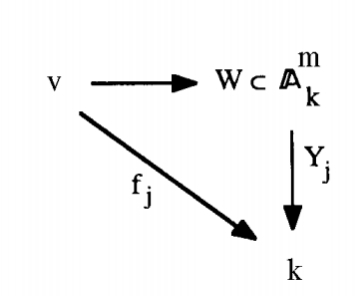
\includegraphics[width=5cm]{68.jpg}\\
		 % \caption{初}
		\end{figure}


		$"\Longrightarrow"$
		如果f是由$F_{1}\cdots,F_{m}$定义的, 那么复合映射就是$P\rightarrow F_{j}(P)$, 是一个多项式函数.

		$"\Longleftarrow"$
		如果$\forall  j, f_{j}\in k[V] $, 那么可以在满足$f_{j}=F_{j} mod I(v), F_{j}\in k[X_{1},X_{2}\cdots,X_{n}]$的$F_{j}$中选一个,就得到了f的一种定义$(F_{1},F_{2}\cdots,F_{m})$

		由这个声明可知, 映射f可写成$f=(f_{1},f_{2}\cdots,f_{m})$.

		多项式映射的复合是由简单的方式定义: 如果$V\subset A^{n}, W\subset A^{m}, U\subset A^{l}$是代数集, 且f:V $\rightarrow $W, g:W $\rightarrow $U 是多项式映射,那么$g\circ f :V \rightarrow U$仍然的一个多项式映射; 如果f是由$F_{1}\cdots,F_{m}\in k[X_{1},X_{2}\cdots,X_{n}]$定义的且g是由$G_{1}\cdots,G_{m}\in k[Y_{1},Y_{2}\cdots,Y_{m}]$定义, 那么$g\circ f$由$G_{1}(F_{1}\cdots,F_{m})\cdots,G_{l}(F_{1}\cdots,F_{m})\in k[X_{1},X_{2}\cdots,X_{n}]$定义

		\textbf{定义} \ 称代数集之间的多项式映射f:V $\rightarrow $W是同构,如果存在多项式映射 g:W $\rightarrow $V使$g\circ f=id_{V}, f\circ g=id_{W}$

		几个多项式映射的例子:(2.1)中的参数化$R^{1}\rightarrow C\subset R^{2}, t\rightarrow (t^{2},t^{3})$或者$(t^{2}-1,t^{2}-t)$, (3.11,b)中讨论的映射$k\rightarrow C\subset A^{3}_{k}, t\rightarrow (t^{3},t^{4},t^{5})$都是多项式映射.并且,在讨论诺特正规化定理时,考虑一个代数集$V\subset A^{n}_{k}$和由m个$Y_{1},Y_{2}\cdots,Y_{m}$的线性形式定义的映射$p:V\rightarrow A^{m}_{k}$, 因为$Y_{i}$是$X_{i}$的线性形式,所以这是多项式映射.

	\section{多项式映射和k[V]}
		\textbf{定理} \ $V\subset A^{n},W\subset A^{m}$是代数集.

		(I)一个多项式映射f:V $\rightarrow $W导出一个环同态$f^{*}:k[W]\rightarrow k[V]$, 是由复合函数定义的, 即如果$g\in k[W]$是多项式函数, 那么$f^{*}(g)=g\circ f$, 并且$g\mapsto g\circ f$定义了一个环同态, 事实上是一个k—代数同态$f^{*}:k[W]\rightarrow k[V]$.

		(II)反过来, 任意一个k—代数同态$\Phi:k[W]\rightarrow k[V]$都是由一个多项式映射f:V $\rightarrow $W唯一定义的,即$\Phi=f^{*}$.

		因此(I)和(II)表明
		\center  $\{$多项式映射$f:V \rightarrow W \}\longrightarrow $$\{$k-代数同态$\Phi:k[W]\rightarrow k[V]\}$



			  $ f \longmapsto f^{*}$

		\justifying


		是双射.

		(III)如果f:V $\rightarrow $W和g:W $\rightarrow $U是多项式应映射, 那么两个环同态可复合$(g\circ f)^{*}=f^{*}\circ g^{*}:k[U]\rightarrow k[W]$

		\textbf{证明} \ (I)通过(4.3), $f^{*}(g)$是多项式映射$V\rightarrow k$, 因此$f^{*}(g)\in k[V]$.显然 $f^{*}(a)=a, \forall a\in k$(这里把k看做V,W上的常值函数).最后 $f^{*}$是环同态是形式上的, 因为k[W]和k[V]是函数环.(环结构是由点态定义的, 例如,$g_{1},g_{2}\in k[W]$, 它们的和 $g_{1}+g_{2}$也是定义在W上是函数且$(g_{1}+g_{2})(P)=g_{1}(P)+g_{2}(P) \forall P\in W$; 所以$f^{*}(g_{1}+g_{2})(Q)=(g_{1}+g_{2})(f(Q))= g_{1}(f(Q))+g_{2}(f(Q))= f^{*}g_{1}(Q)+f^{*}g_{2}(Q))$

		(III)可由映射的复合推导出

		(II)的证明需要更多的技巧, 对于$i=1,2\cdots,m$, 令$y_{i}\in k[W]$是W上的第i个坐标函数,所以
		\begin{equation*}
		k[W]=k[y_{1}  \cdot, y_{m}]=k[Y_{1},Y_{2} \cdots,Y_{m}]/I(W)
		\end{equation*}
		现在$\Phi:k[W]\rightarrow k[V]$已经给出, 所以可以$f_{i}=\Phi(y_{i})$定义$f_{i}\in k[V]$

		考虑映射$f:V \rightarrow A^{m}_{k}, f(P)=f_{1}(P)\cdots f_{m}(P)$, 由于$f_{i}\in k[V]$, 所以f是多项式映射, 进一步f把V嵌入到W中,即$f(V)\subset W$.事实上, 假设$G\in I(W)\subset k[Y_{1},Y_{2}\cdots,Y_{m}]$; 那么
		\begin{equation*}
		G(y_{1}\cdot ,y_{m})=0\in k[W]
		\end{equation*}
		左边是我把环元素$y_{i}$代入多项式表达式G, 所以$\Phi(G(y_{1}\cdot y_{m}))=0\in k[V]$; 但k是k-代数同态, 所以
		\begin{equation*}
		k[V]\in0=\Phi(G(y_{1}\cdot, y_{m}))=G(\Phi(y_{1})\cdot ,\Phi(y_{m}))=G(f_{1}\cdot ,f_{m})
		\end{equation*}
		$f{i}$是V上的函数, $G(f_{1}\cdot f_{m})\in k[V]$是由函数$P\mapsto G(f_{1}(P))\cdot ,f_{m}(P))$定义的. 这证明了对$P\in V$,每一个$G\in I(W),f(P)$的坐标($f_{1}(P))\cdot ,f_{m}(P)$)满足$G(f_{1}(P))\cdot ,f_{m}(P))=0$.因为W是由$G\in I(W)$的零点定义的$A^{m}_{k}$的子集,它满足$f(P)\in W$. 这证明了上面给出分f是多项式映射f:V $\rightarrow $W.为了检验两个k-代数同态$f^{*},\Phi:k[W]\rightarrow k[V]$相符, 只要证明它们的生成元相同,即$f^{*}(y_{i})=\Phi(y_{i})$,从f的构造中可以发现这个事实.一个相似的论证可以表明映射f是由$f^{*}(y_{i})=\Phi(y_{i})$  唯一决定的.
	\section{推论}一个多项式映射f:V $\rightarrow $W是同构当且仅当$f^{*}:k[W]\rightarrow k[V]$是同构.

		\textbf{例子} \ k是无限域,多项式映射
		\begin{equation*}
		\varphi:A^{1}_{k}\rightarrow C:(Y^{2}=X^{3})  T\mapsto (T^{2},T^{3})
		\end{equation*}
		不是同构.因为这种情况下, 同态
		\begin{equation*}
		\varphi^{*}:k[C]=k[X,Y]/(Y^{2}-X^{3})\rightarrow k[T]
		\end{equation*}
		是由$X\mapsto T^{2},Y\mapsto T^{3}$给出的.$\varphi^{*}$的象是由$T^{2},T^{3}$生成的k-代数,$k[T^{2},T^{3}]\subsetneq k[T]$
		注意到$\varphi$是双射,所以有一个逆映射$\psi :C\rightarrow A^{1}_{k}$,如果X=Y=0,则$(X,Y)\mapsto 0$, 否则$(X,Y)\mapsto Y/X$.所以$\varphi$为什么不是同构呢?重点是C上的多项式比$A^{1}_{k}$上的少.
	\section{仿射簇}
		k是一个域, 仿射簇是同构意义下的不可约代数集$V\subset A^{n}_{k}$.

		定理4.4告诉我们坐标环k[V]是V的同构类中的不变量.这样我就可以少用$V\subset A^{n}_{k}$周围的空间定义簇;后面提出的仿射簇总是上述意义下的.

		\textbf{定义} \ k上的仿射簇是集合V和环k[V], 其中的k-值函数$f:V\rightarrow k$ 满足

		(i)k[V]是有限生成的k-代数,

		(ii)从k[V]选择一些生成元$x_{1}  \cdot, x_{n}$,映射
		\center $ V \rightarrow  A^{n}_{k}$


		$P\mapsto x_{1}(P)  \cdot, x_{n}(P)$

		\justifying
		把V作为不可约代数集嵌入到 $A^{n}_{k}$.
		\section{函数域}V是仿射簇, 那么V的坐标环k[V]是整环,其中的函数是V上的k值函数.

		\textbf{定义} \ V的函数域k(V)是分式域,k(V)=k[V]的商环Quot(k[V]).一个元素$f\in k(V)$是V上的有理函数;$f\in k(V)$是由f=g/h定义的,其中$g,h\in k[V]$且$h\neq 0$.

		先验f不是V上的函数,因为在h的零点处f无定义, 可是f在$P\in V,h(P)\neq 0$处有定义,所以f至少是一个“部分定义函数”,下面介绍一些术语支持这个想法.

		\textbf{定义} $f\in k(V),P\in V$, 称f是正则的或者P在f的定义域内, 如果存在一种表达f=g/h, 其中$g,h\in k[V]$且$h(P)\neq 0$.

		值得注意的是k[V]通常不是UFD,所以$f\in k(V)$可能有本质不同的表示法f=g/h, 见习题4.9中的例子.

		称

		\center  $dom \ f=\{P\in V\vert f$在P点正则$\}$为f的定义域.

						且$V,P=\{f\in k(V) \vert f$在P点正则$\}=k[V][\{h^{-1}\vert h(P)\neq 0\}]$

		\justifying
		那么$V,P\subset k(V)$是子环,是V在P点的局部环.
	\section{定理}
		(I)dom f在Zariski拓扑下是稠密的开集.

		假设k是代数闭域;那么

		(II)$dom \ f=V\iff f\in k[V]$(即多项式函数=正则有理函数),

		进一步,对任意的$h\in k[V]$,令
		\begin{equation*}
		V_{h}=V\backslash V(h)=\{P\in V \vert h(P)\neq 0\}
		\end{equation*}
		那么(III)$V_{h}\subset dom \ f \iff f\in k[V][h^{-1}]$.

		\textbf{证明} \ 定义$f\in k(V)$的分母的理想

		\center $ D_{f}=\{ h\in k[V] \vert hf\in k[V] \}\subset k[V]$




			  $ =\{ h\in k[V] \vert$ 存在一个表示f=g/h, 其中$g\in k[V]\cup \{0\}$

		\justifying

		从第一行可以看出, $D_{f}$是k[V]的理想.证明:

		\begin{equation*}
		V\backslash dom \ f=\{P\in V \vert h(P)= 0 \forall h\in D_{f}\}=V(D_{f})
		\end{equation*}
		所以$V\backslash dom \ f$是V的代数集,因此$dom \ f=V\backslash V(D_{f})$是闭集的补集,所以是Zariski拓扑下的开集. dom \ f显然是非空的,所以由推定理4.2知是稠密的.

		使用零点定理的(b),
		\begin{equation*}
		dom f=V\iff V(D_{f})=\emptyset \iff 1\in D_{f} \iff f\in k[V]
		\end{equation*}
		最后,

		$V_{h}\subset dom \ f \iff h $在$V(D_{f})$上为0,

		使用零点定理的(c),$\iff h^{n}\in D_{f}$,对某些n,即$f=g/h^{n}\in k[V][h^{-1}]$

	\section{有理映射}V是仿射簇

		\textbf{定义} \ 一个有理映射$f:V\rightarrow A^{n}_{k}$是由有理函数$f_{1}\cdots ,f_{n}$部分定义的映射,即

		\begin{equation*}
		f(P)=(f_{1}(P)\cdots, f_{n}(P)) \forall P\in \cap dom \ f_{i}
		\end{equation*}

		通过定义,$dom \ f=\cap dom \ f_{i}$, 称f在P点是正则的当且仅当$P\in dom f$. 两个仿射簇$V\subset A^{n},W\subset A^{m}$之间的有理映射$V\rightarrow W$被定义成有理映射$f:V\rightarrow A^{m}$,满足$f(dom \ f)\subset W.$

		在(4.3)的结尾有两个有理映射的例子.

	\section{有理映射的复合映射}
		有理映射f:V $\rightarrow $W和g:W $\rightarrow $U的复合映射$(g\circ f)$可能没有定义.这个困难是由有理映射不是映射造成的,显然复合映射定义在$dom \ f\cap f^{-1}(dom \ g)$; 可是这很可能是空集(见练习4.10)

		在代数表示上,相同的问题也会发生:假如f是由$f_{1}\cdots ,f_{m}\in k(V)$给出, 那么
		\begin{equation*}
		f:V \rightarrow W\subset A^{m}
		P \mapsto f_{1}(P)\cdots, f_{m}(P)
		\end{equation*}
		对$P\in \cap dom \ f_{i}$;任意的$g\in k[W]$是 $g=G \ mod \ I(W)$ 的形式, 对一些$G\in k[Y_{1}\cdots,Y_{m}]$且$g\circ f=G(f_{1}\cdots ,f_{m})$ 在k(V)上是定义良好的. 所以想(4.4)一样,有一个k-代数同态
		\begin{equation*}
		f^{*}:k[W]\rightarrow k(V)
		\end{equation*}
		对应f.可是,如果$h\in k[W]$是$f^{*}$的kernel, $f^{*}(g/h)$可能没意义,所以$f^{*}$不能延拓到域同态$k(W)\rightarrow k(V)$

		\textbf{定义} \ 称$f:V \rightarrow W$是dominant如果f(dom \ f)在W中在Zariski拓扑下是稠密的.

		几何上,这意味着对任意的有理映射$g:W\rightarrow U,  f^{-1}(dom \ g)\subset dom \ f$是稠密的开集,所以$g\circ f$定义在V上的稠密的开集上,所以是部分定义的映射$V\rightarrow U$.

		代数上,

		\center  f是dominant $\iff f^{*}k[W]\rightarrow k(V)$是单射

		\justifying
		对给定的$g\in k[W]$,
		\begin{equation*}
		g\in ker f^{*} \iff f(dom f)\subset V(g)
		\end{equation*}

		即$f^{*}$不是单射当且仅当f(dom \ f)是W的真子集.

		显然,有理映射f和g的复合映射$g\circ f$中f是dominant,$g\circ f$是有理映射,由$f^{*}(g_{i})$组成.注意到$g\circ f$的定义域包含 $f^{-1}(dom \ g)\cap dom f$, 但可能会更大(见习题4.6)
	\section{定理}
		(I)一个dominant的有理映射$f:V\rightarrow W$定义一个域同态$f^{*}:k(W)\rightarrow k(V)$.

		(II)反过来,一个k-同态$\Phi: k(W)\rightarrow k(V)$来自一个唯一定义的有理映射$f:V\rightarrow W$.

		(III)如果f和g是dominant的,则$(g\circ f)^{*}=f^{*}\circ g^{*}$

		证明仅仅需要(4.4)做微小的变动.

	\section{来自仿射簇开集的态射}
		V,W是仿射簇,$U\subset V$是开集.

		\textbf{定义} \ 态射$f:V\rightarrow W$是有理映射$f:V\rightarrow W$满足$U\subset dom f$,所以f在每一点$P\in U$是正则的.

		如果$U_{1}\subset V,U_{2}\subset W$是开集那么一个态射$f:U_{1}\rightarrow U_{2}$就是一个态射$f:U_{1}\rightarrow W$,满足$f(U_{1})\subset U_{2}$. 同构是指一个态射两边都有逆态射.

		如果V,W是仿射簇,那么由同构定理(4.8II)
		\center  $\{$态射$f:V\rightarrow W\}=\{$多项式映射$f:V\rightarrow W\}$


		\justifying
		\textbf{例子} \ (2.1)中的三次曲线参数化$A^{1} \rightarrow C:(Y^{2}=X^{3}) $导出同态$A^{1}\backslash \{0\}\backsimeq C\backslash \{0,0\}$,细节见练习4.5.


	\section{标准的开集}


		\textbf{定理} \ $V_{f}$是到仿射簇的同构,且$k[V_{f}]=k[V][f^{-1}].$

		\textbf{证明}想法是考虑函数$f^{-1}$的图像;使用(3.10)中NSS$(b)\Rightarrow(c)$证明中相似的方法.
		\begin{figure}[h]
		  \centering
		  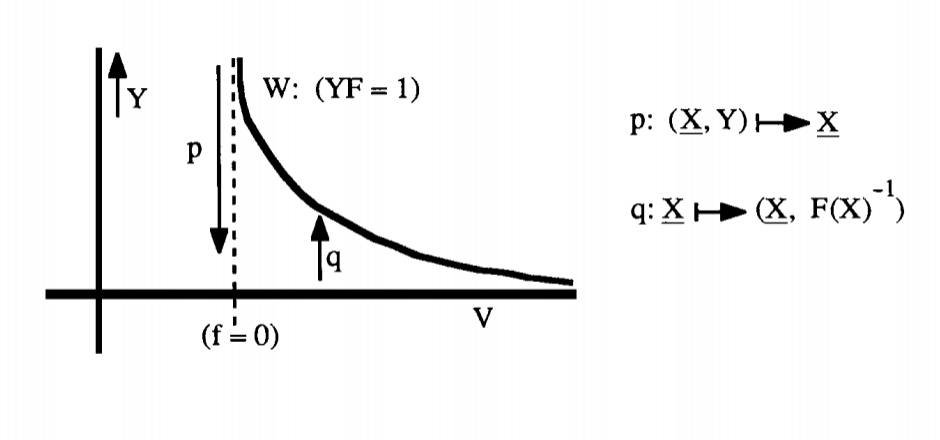
\includegraphics[width=10cm]{75.jpg}\\
		 % \caption{初}
		\end{figure}

		$J=I(V)\subset k[X_{1},X_{2}\cdots,X_{n}]$,选择$F\in k[X_{1},X_{2}\cdots,X_{n}]$使$f=F \ mod \ I(V)$.现在定义$I=(J,YF-1)\subset k[X_{1},X_{2}\cdots,X_{n},Y]$,令$V(I)=W\subset A^{n+1}.$
		很容易检验图中的映射是$V_{f}$和W之间的可逆态射,关于坐标环的说明在(4.8,III).

		标准开集$V_{f}$是很重要的, 因为它形成了V的Zariski拓扑的一组基:每一个开集$U\subset V$都是一些$V_{f}$的并集(因为每一个闭集的形式都是$V(I)=\cap_{f \in I} V(f)$).因此结果就证明了每一个开集$U\subset V$都是仿射簇开集$V_{f}$的并集.



\chapter{射影几何和双有理几何}
	本章节的第一部分旨在概括第三章和第四章关于射影簇的内容.剩下的部分主要关于双有理几何,其中用到了第四章最后部分的函数域$ k(V) $,这一部分在射影或者仿射情景下也是适合的.
	
	\setcounter{section}{-1}
	\section{为什么射影簇是簇}
		三次曲线
		\begin{equation*}
		C :\left( Y ^{2} Z = X ^{3}+ aXZ ^{2}+ bZ ^{3}\right) \subset \mathbb{P} ^{2}
		\end{equation*}
		是两个仿射曲线的联合:
		\begin{equation*}
		\left. C _{0}:\left( y ^{2}= x ^{3}+ ax + b \right) \subset \mathbb{A} ^{2} \quad  C \text{中取} (Z = 1) \text{截面}\right)
		\end{equation*}
		和
		\begin{equation*}
		\left. C _{1}:\left( z _{1}= x _{1}^{3}+ axz _{1} 2+ bz _{1}^{3}\right) \subset \mathbb{A} ^{2}   C \text{中取} (Y = 1) \text{截面}\right)
		\end{equation*}
		这种联合由同构
		\begin{equation*}
		C _{0} \backslash( y =0) \longrightarrow  C _{1} \backslash\left( z _{1}=0\right)
		\end{equation*}
		\begin{equation*}
		( x , y ) \mapsto( x / y , 1 / y )
		\end{equation*}
		所胶合的.
		
		
		作为一个较为简单的例子, 有着齐次坐标 $( X , Y )$的$\mathbb{P}^{1}$是两个分别具有坐标$ x_{0},y_{1} $的 $\mathbb{A}^{1}$的联合,这种联合由同构
		\begin{equation*}
		\mathbb{A}^{1} \backslash\left(x_{0}=0\right)\rightarrow \mathbb{A}^{1} \backslash\left(y_{1}=0\right)
		\end{equation*}
		\begin{equation*}
		x _{0} \quad \mapsto \quad 1 / x _{0}
		\end{equation*}
		所胶合的.
		
		
		\begin{figure}[h]
			\centering
			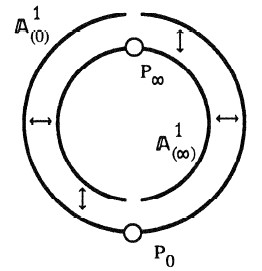
\includegraphics[width=5cm]{50.jpg}\\
			\caption*{一个简单的图例,其中'$ \leftrightarrow $'代表同构}
		\end{figure}
	
		
		重点是,这种簇是严格大于仿射簇的. 事实上,根据之后会提到的自然态射的概念, 可以看出不存在非恒定态射$\mathbb{P} ^{1} \rightarrow \mathbb{A} ^{n}$或$C \rightarrow \mathbb{A}^{n}$ 对于任意的$n$ (可见\textit{习题5.1}和\textit{习题5.12},在(8.10)中也有讨论).
		
		
		解决该问题的一种方法是采用适当的模来胶合,而将“抽象簇” $ V $的概念定义为仿射簇的并集$ V = \ cup V _ {i} $.类似于拓扑中流形的定义,这是一个有吸引力的想法,但是它带来了更多的技术难题。使用射影簇可以通过在现成的环绕空间$ P ^ {n}$中工作来避免这些问题,因此(除了对齐次多项式有所了解之外),它们比仿射簇更难研究。实际上,尽管在初级阶段可能还不清楚,但是射影簇在相当可观的范围内为研究簇提供了自然的框架(在(8.11)中有从更高层次的简单论述)。
		
	\section{分次环和齐次理想}
		\textbf{定义}\ 一个多项式$f \in k \left[ X _{0} \ldots X _{ n }\right]$是$ d $次齐次的,如果
		\begin{equation*}
			f =\sum a _{ i _{0}} \cdot i _{ n } X _{0}^{ i _{0}} \ldots X _{ n }^{ i _{ n }} \text{其中} a _{ i _{0}} \ldots i _{ n } \neq 0 \text{当且仅当} i _{0}+\ldots i _{ n }= d
		\end{equation*}
		对于任意$f \in k \left[ X _{0} \ldots X _{ n }\right]$存在一个唯一的表达$f = f _{0}+ f _{1}+\ldots f _{ N }$ 其中$f _{ d }$ 是具有$ d $次齐次的多项式,而$d =0,1, \ldots N$.
		
		
		\textbf{命题}\ 如果$f$ 是$ d $次齐次的,则
		\begin{equation*}
		f \left(\lambda X _{0}, \ldots \lambda X _{ n }\right)=\lambda d f \left( X _{0}, \ldots X _{ n }\right) \quad \text { for all } \quad \lambda \in k
		\end{equation*}
		如果$k$是一个无限域,则反之亦成立.
		
		
		\textbf{证明}\ 
		
		
		\textbf{定义}\ 一个理想$I \subset k \left[ X _{0}, \ldots X _{ n }\right]$是齐次的,如果对于所有$f \in I$,在$ f $的齐次分解$f = f _{0}+ f _{1}+\ldots f _{ N }$中,对于所有$ i $有$f _{ i } \in I$.
		
		
		这等价于$ I $是由(有限个)齐次多项式生成的.
		
		
	\section{齐次的$ V-I $对应}
		取$\mathbb{P} ^{n}_{k}$ 是一个在域$ k $上的$ n- $维射影空间,其中有齐次坐标$X _{0} . . X _{ n }$.则$f \in k \left[ X _{0}, \ldots X _{ n }\right]$不是一个在$\mathbb{P} ^{ n } k $上的函数:由定义,$\mathbb{P} ^{ n }_{ k }= k ^{ n +1} \backslash\{0\} / \sim$,其中$\sim$是一个等价关系,这个等价关系是$\left( X _{0}, \ldots X _{ n }\right) \sim\left(\lambda X _{0}, \ldots \lambda X _{ n }\right)$其中$\lambda \in k \backslash\{0\} $;而$ f $是一个在$k ^{n+1}$上的函数.但是,对于$P \in \mathbb{P}^{n} ,$如果$ f $是齐次的,那么条件$f ( P )=0$就是良定义的:假设$P =\left( X _{0}: . X _{ n }\right)$,则$\left(X_{0}, \ldots X_{n}\right)$是$ P $在 $k^{n+1} \backslash\{0\}$上的等价类的代表元.因为$f(\lambda \underline{X})=\lambda^{d} f(\underline{X}),$如果$f\left(X_{0}, \ldots X_{n}\right)=0$ 那么就有$f\left(\lambda X_{0}, \ldots \lambda X_{n}\right)=0,$因此条件$f ( P )=0$是独立于代表元的选取的.出于这种想法像以前一样定义对应$ V,I $
		\begin{equation*}
		\left\{\text {齐次理想 } J \subset k \left[ X _{0}, \dots X _{ n }\right]\right\} \quad \stackrel{ V , I }{\longleftrightarrow}\left\{\text { 子集} X \in \mathbb{P} _{ k }\right\}
		\end{equation*}
		其中
		\begin{equation*}
		V ( J )=\left\{ P \in \mathbb{P} ^{ n } k | f ( P )=0 \forall \text { 齐次} f \in J \right\}
		\end{equation*}
		\begin{equation*}
		I ( X )=\left\{ f \in k \left[ X _{0}, \ldots X _{ n }\right] |  \text { 对于所有 } P \in X \text{有} f ( P )=0\right\}
		\end{equation*}
		作为一个练习,想一想为什么 $I ( X )$ 是一个齐次理想.
		对应$ V $和$ I $满足仿射条件下的$ V,I $的一样形式的属性(例如$V \left( J _{1}+ J _{2}\right)=  V \left( J _{1}\right) \cap V \left( J _{2}\right) $依然成立). $V ( I )$的子集是$\mathbb{P}^{n} _{ k }$的代数子集,类似在仿射条件下的结论,如果在 $\mathbb{P} ^{n}_{k}$上定义代数子集是闭集就能构造一个Zariski拓扑.
		
		
	\section{射影条件下的零点定理}
		 As with the affine correspondences, it is purely formal that $I ( V ( J )) \supset$ rad $J$ for any ideal $J ,$ and that for an algebraic set,
		(1) $= k \left[ X _{0} \ldots X _{ n }\right]$ (the whole ring) defines the empty set in $k ^{ n +1},$ hence also in $P ^{n}_{ k },$ which is as it should he; however, the ideal $\left(X_{0} \ldots X_{n}\right)$ defines $\{0\}$ in $k ^{n+1}$ which also corresponds to the empty set in $P ^{n}_{ k }$. The ideal $\left(X_{0}, \ldots X_{n}\right)$ is an
\end{document}
